%! TEX root = ./thesis.tex
\chapter{Suchprobleme und die Hypothese $\hQ$ im Kontext des Pudlákschen Programms}\label{chap:pudlak}


In der Einleitung dieser Arbeit wurde bereits angedeutet, dass die Hypothese $\hQ$ von \citeauthor{fenner_inverting_2003} große Nähe und Verwandtschaft zu Hypothesen hat, die Suchprobleme im Allgemeinen und Beweissystemen im Speziellen betreffen. Damit ergeben sich Beziehungen zu Hypothesen aus dem Pudlákschen Programm, insbesondere $\neg\hSAT$ (also dass eine NP-vollständige Mengen mit $\P$-optimalem Beweissystem für diese Menge existiert).
In diesem Kapitel werden wir diese Beziehungen näher erarbeiten. Zur Erinnerung:

\begin{reptheorem}{Vermutung}{conj:q}[$\hQ$, \cite{fenner_inverting_2003}]
    Für jede totale NPTM $N$ (d.h. $L(N)=\Sigma^*$) existiert eine Funktion $g\in\FP$ sodass für alle $x$ das Bild $g(x)$ ein akzeptierender Rechenweg von $N(x)$ ist. 
\end{reptheorem}


Im Kapitel werden wir uns grob folgenden drei Desiderata widmen: 
erstens, nähern wir uns in Abschnitt~\ref{sec:karp-vs-levin} erneut der Frage zwischen Levin- und Karp-Vollständigkeit bzw. der Hypothese $\mathsf{KvL}$ aus vorigem Kapitel. Insbesondere analysieren wir die Beziehungen von $\mathsf{KvL}$ zu $\hQ$ und versuchen, $\mathsf{KvL}$ in das Pudláksche Programm einzuordnen.

Zweitens, in Abschnitt~\ref{sec:q-vs-search}, verallgemeinern wir Charakterisierungen von $\hQ$, die sich insbesondere auf Suchprobleme und deren assoziierte Beweissysteme beziehen.
Insbesondere zeigen wir für die vollständigen NP-Suchprobleme $R$ dass das zu $R$ assoziierte \emph{Standardbeweissystem} ($(x,y)$ mit $R(x,y)$ ist ein Standardbeweis für $x$) $\P$-optimal ist, genau dann wenn $\hQ$. Damit wird die $\P$-Optimalität des entsprechenden Standardbeweissystems zu einer Invariante, die entweder für \emph{alle} vollständigen NP-Suchprobleme zutrifft, oder für \emph{keins}.

%erstens werden wir weitere Hypothesenzu Suchproblemen, welche sich im Verlauf dieser Arbeit ergeben, in das Pudláksche Programm einordnen, insbesondere $\hQ$ und $\mathsf{KvL}$ bzw. die Frage nach Levin- vs. Karp-Vollständigkeit.
%Im Speziellen ergänzen wir das Abbildung~\ref{fig:pudlak} der Beziehungen zwischen den Pudlákschen Hypothesen aus der Einleitung um weitere Hypothesen, und erreichen Abbildung~\ref{}. Die Beweise 

%Zweitens eine Verallgemeinerung der Charakterisierung $\hQ$, die sich insbesondere auf Suchprobleme und deren Beweissysteme bzw. „Zertifikatsschemata“ beziehen.

\looseness=1
Drittens ergänzen wir im gesamten Verlauf dieses Kapitels das Pudláksche Programm um weitere Hypothesen ($\mathsf{KvL}, \hQ, \dots$), sodass Abbildung~\ref{fig:pudlak-small} der Beziehungen zwischen den Pudlákschen Hypothesen vergrößert wird. Damit erreichen wir den Stand, der in Abbildung~\ref{fig:figure-implications} dargestellt wird.
Damit einher wird abschließend ein Überblick über Orakel angegeben, welche Hypothesen des Pudlákschen Programms (ergänzt um $\hQ, \mathsf{KvL}, \dots$) trennen.


Für alle dieser drei Desiderata ist es zunächst notwendig, auf die Hypothese $\hQ$ einzugehen.
\textcite{fenner_inverting_2003} beobachten, dass das Invertieren von surjektiven ehrlichen FP-Funktionen eine erstaunlich robuste Aussage ist, die eine Vielzahl von äquivalenten „fundamentalen“ \parencite{fenner_inverting_2003} Charakterisierungen aus der Komplexitätstheorie zulässt, so zum Beispiel die effiziente Lösbarkeit von TFNP-Suchproblemen, oder das effiziente Ausrechnen akzeptierender Rechenwege einer totalen NPTM. Wir können jetzt schon festhalten, dass die aktuelle Forschung diese Hypothese als sehr stark einschätzt, und eher die negative Beantwortung $\neg\hQ$ vermutet.


\begin{theorem}[Äquivalente Formulierungen der Hypothese $\hQ$; \cite{fenner_inverting_2003}]\label{thm:q-orig}
    Folgende Aussagen sind äquivalent:
    \begin{enumerate}
        \item Hypothese $\hQ$.
        \item $\mathrm{NPMV}_t\subseteqc \mathrm{FP}$.
        \item $\TFNP\subseteqc \mathrm{FP}$.
        \item $\P=\NP\cap\coNP$ und $\mathrm{NPMV}_t\subseteqc \mathrm{NPSV}_t$.
        \item Jede surjektive ehrlichen Funktion $f\in\FP$ ist $\P$-invertierbar.
        \item Für jede Menge $L\in \P$  und jede NPTM $N$ mit $L(N)=L$ existiert eine Funktion $h\in \FP$ mit 
            \[ x\in L \implies N(x) \text{ akz. mit Rechenweg $h(x)$}. \]
    \end{enumerate}
\end{theorem}
Dieser Satz relativiert insbesondere.

\textcite{fenner_inverting_2003} und \textcite{kobler_is_2000} charakterisieren $\hQ$ noch durch zwei weitere Formen, diesmal über je eine Aussage über die Menge $\mathtt{SAT}$:

\begin{theorem}[\cite{fenner_inverting_2003}]\label{thm:q-fenner}
    Es gilt $\hQ$ genau dann wenn Folgendes gilt: Für jede NPTM $N$ mit $L(N)=\mathtt{SAT}$ existiert eine Funktion $h\in \FP$ sodass 
\[ N(\phi) \text{ akz. mit Rechenweg $w$} \implies \text{$h(w)$ ist eine erfüllende Belegung für $\phi$.} \]
\end{theorem}
\begin{theorem}[\cite{kobler_is_2000}]\label{thm:q-messner}
    Es gilt $\hQ$ genau dann wenn das Standardbeweissystem $\mathit{sat}$
            \[ \mathit{sat}(\phi, w) = \begin{cases} \phi & \text{wenn $w$ eine erfüllende Belegung für $\phi$ ist} \\ \bot & \text{sonst.} \end{cases}\]
            für $\mathtt{rSAT}$ $\P$-optimal ist.
\end{theorem}
Diese zwei Sätze relativieren nicht.

\begin{figure*}[p]
    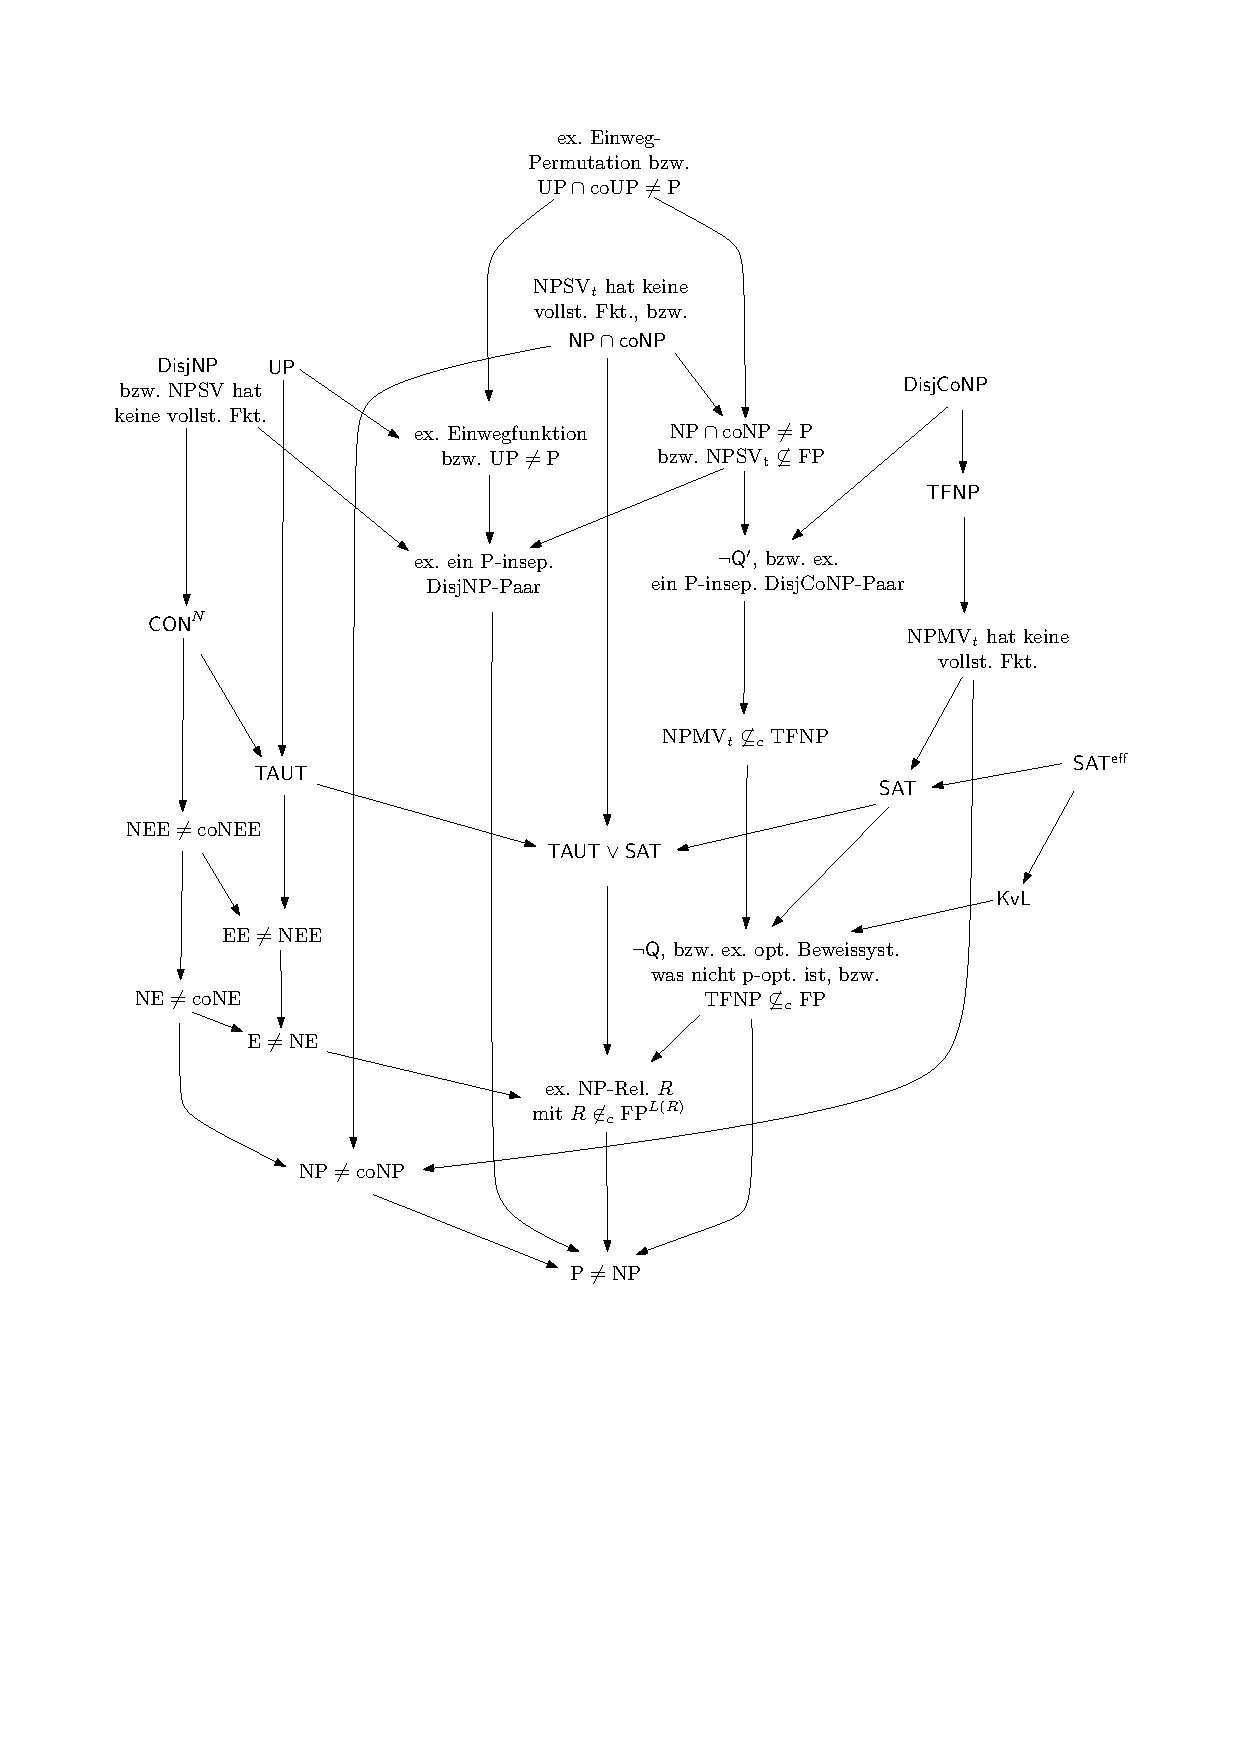
\includegraphics[page=1]{figures.pdf}
    \caption{Bekannte (relativierenden) Implikationen zwischen den betrachteten Hypothesen und weiteren Aussagen. Satz~\ref{thm:figure-implications} gibt Belegstellen für jede dieser Implikationen an.}\label{fig:figure-implications}
    \forcerectofloat
\end{figure*}

In anderen Worten sagt Satz~\ref{thm:q-fenner} aus, dass unter Annahme von $\hQ$ es modulo Umcodieren nur einen einzigen SAT-Solver gibt, und insbesondere alle SAT-Solver äquivalent zum trivialen Solver sind, welcher nur alle möglichen Belegungen ausprobiert.
Satz~\ref{thm:q-messner} macht eine analoge Aussage über Beweissysteme: egal wie komplex ein Beweissystem $h$ für $\mathtt{SAT}$ ist, wir können immer einen $h$-Beweis für $\phi$ in eine erfüllende Belegung für $\phi$ (quasi ein trivialer Beweis für $\phi\in\mathtt{SAT}$) transformieren. Damit ist auch leicht zu sehen, dass $\hQ\Rightarrow \neg\hSAT$, zumindest im unrelativierten Fall.

In Abschnitt~\ref{sec:q-vs-search} werden wir sehen, dass sich die obigen Charakterisierungen auf weitere (aber möglicherweise nicht alle) vollständigen NP-Relationen generalisiert, womit insbesondere auch die beiden Charakterisierungen von \citeauthor{fenner_inverting_2003} und \citeauthor{kobler_is_2000} zu einer \emph{relativierbaren} Variante verallgemeinert werden.
Mit dieser Verallgemeinerung ist es dann auch für uns möglich, $\hQ$ formal in das Pudláksche Programm (u.a. durch $\hQ\Rightarrow \neg\hSAT$) einzuordnen. Hierfür führen wir jetzt schon den Begriff eines Standardbeweissystems formal ein.

\begin{definition}[Standardbeweissystem einer NP-Relation]
    Sei $R$ eine NP-Relation. Wir definieren bezüglich $R$ das \emph{Standardbeweissystem} $\mathit{std}_R$ für $\Proj(R)$ wie folgt:
    \[ \mathit{std}_R(w) \defeq \begin{cases} x & \text{wenn $w=(x,y)$ und $(x,y)\in R$,}\\
    \bot & \text{sonst}.\end{cases} \qedhere \] 
\end{definition}
Damit ist, wie durch die Formulierung oben suggeriert, $\mathit{sat}=\mathit{std}_{\mathtt{rSAT}}$.
Bevor wir nun mit einer Diskussion zwischen Karp-Vollständigkeit und Levin-Vollständigkeit fortsetzen, schließen wir diesen Einstieg mit folgender einfachen Beobachtung ab:
\begin{observation}\label{obs:spps-honest}
    Für jede NP-Relation $R$ ist das Standardbeweissystem $\mathit{std}_R$ für $\Proj(R)$ ehrlich, optimal, und hat kurze Beweise.
\end{observation}
\begin{proof}
    Nachdem $R$ polynomiell längenbeschränkt ist, folgt sofort dass $\mathit{std}_R$ kurze Beweise hat. 
    Nach Beobachtung \ref{obs:super-ps-sind-opt} damit auch optimal.
    Insbesondere hat $\mathit{std}_R$ \emph{nur} polynomiell längere Beweise, also ist $\mathit{std}_R$ ehrlich.
\end{proof}
%\begin{proof}
    %Sei $q$ die Zertifikatsschranke von $R$, und sei $w=(x,y)$ gegeben sodass $\mathit{std}_R(x,y) = x$.
    %An dieser Stelle müssen wir auf die konkrete Codierung von Beweisen $w=(x,y)$ eingehen.
    %Wie in \ref{sec:notation} beschrieben, codieren wir Tupel in einer solchen Weise sodass
    %\[ |w| = |(x,y)| = 2(|x|+|y|+2) = 2|x|+ 2|y| + 4. \]
    %Da $(x,y)\in R$ gilt für $y$ auch $|y|\leq q(|x|)$.
    %Damit also
    %\[ |w| \leq 2|x|+ 2q(|x|) + 4 \leq q'(|x|) = q'(|\mathit{std}_R(w)|). \]
    %für ein geeignetes Polynom $q'$, wie gewünscht.
%\end{proof}

\section{Karp-Vollständigkeit vs. Levin-Vollständigkeit}\label{sec:karp-vs-levin}

Wir wiederholen hier erneut die zentrale offene Frage und Vermutung aus Abschnitt~\ref{sec:levin}:

\begin{reptheorem}{Frage}{question:kvl}
Wenn $\Proj(R)$ eine $\leqmp$-vollständige Menge für $\NP$ ist, ist dann auch $R$ eine $\leqlp$-vollständige NP-Relation für $\FNP$?
\end{reptheorem}

\begin{reptheorem}{Vermutung}{conj:kvl}[$\mathsf{KvL}$]
    Es existiert eine NP-Relation $R$ sodass $\Proj(R)$ $\leqmp$-vollständig für $\NP$ ist, aber $R$ ist nicht $\leqlp$-vollständig für $\FNP$.
\end{reptheorem}

Zunächst sei hier noch einmal hervorgehoben, dass eine Beantwortung der Frage~\ref{question:kvl} schwer ist. Zum einen haben wir bereits gesehen, dass ein Beweis $\mathsf{KvL}$ auch sofort $\P\neq\NP$ beweisen würde. Insbesondere ist ein relativierender Beweis von $\mathsf{KvL}$ ausgeschlossen, denn existiert ein Orakel, relativ zu diesem $\neg\mathsf{KvL}$ (z.B. ein PSPACE-vollständiges Orakel, welches $\NP$ auf $\P$ kollabiert).

Wir werden uns daher im Folgenden insbesondere auf Beziehungen zwischen $\mathsf{KvL}$ und gewissen anderen Hypothesen konzentrieren.
In diesem Sinne möchte ich argumentieren, dass die obige Frage bzw. Vermutung eng mit der Hypothese $\hQ$ zusammenhängt.
Im Speziellen werden wir sehen, dass die Hypothese $\hQ$ so charakterisiert werden kann, dass sie einer Verstärkung der Vermutung $\neg\mathsf{KvL}$ entspricht.\footnote{\textcite{fenner_inverting_2003} gaben hierbei eine ähnliche Aussage an (Cor.~3: „$\hQ$ holds iff every Karp reduction from $A$ to $B$ can be extended to a Levin reduction“), es ist aber hervorzuheben, dass die Autoren von einem unüblichen Begriff von Levin-Reduktionen ausgehen, der sich von dem hier verwendeten unterscheidet. Dieser umfasst nicht eine „Rückwärts-Translation“ von Zertifikaten für $B$-Instanzen zu $A$-Instanzen, sondern eine „Vorwärts-Translation“ von Zertifikaten für $A$-Instanzen zu $B$-Instanzen.}

\begin{theorem}\label{thm:q-as-levin}
    Folgende Aussagen sind äquivalent:
    \begin{enumerate}
        \item Hypothese $\hQ$, bzw. $\TFNP\subseteqc\FP$. 
        \item Für jedes Paar von NP-Relationen $A, B$ gilt:
            \[ \Proj(A) \leqmp \Proj(B) \iff A \leqlp B. \]
    \end{enumerate}
\end{theorem}
\begin{proof}
    \begin{prooflist}
\item (1)$\implies$(2): Die Richtung von rechts nach links ist klar. Für die andere Richtung sei $\Proj(A) \leqmp \Proj(B)$ mit $A,B$ NP-Relationen. Sei $q$ hierbei das Polynom was die Zertifikatslänge in $A$ begrenzt.
    Wir wollen nun eine Levin-Reduktion von $A$ auf $B$ angeben. Sei $f\in \FP$ die Funktion, welche die Reduktion $\Proj(A) \leqmp \Proj(B)$ realisiert.

    Definiere folgende Relation $R$ mit
    \[ \fset{}R(w) = \begin{cases} \{ y\mid y\in\Sigma^{\leq q(|x|)}, (x,y)\in A \} & \text{falls $w=(x,y')$, $(f(x), y')\in B$} \\  \{\epsilon\} & \text{sonst}. \end{cases} \]
    Es ist leicht zu sehen, dass $R$ eine totale NP-Relation ist. Nach (1) existiert nun eine (totale) Verfeinerung $g\in \FP$ von $R$.

    Damit lässt die Levin-Reduktion von $A$ auf $B$ angeben: wähle $f$ als Reduktionsfunktion, und sei die Funktion $g$ von oben die Translationsfunktion. Dann gilt
    \begin{gather*}
        (f(x), y') \in B \implies (x, y')\in\Proj(R) \\
        \implies ((x, y'), g(x, y'))\in R\\
        \implies (x, g(x, y')) \in A \text{ nach Def. von $R$}
    \end{gather*}
    wie gewünscht. Wir haben $A\leqlp$ via $f, g$.
\item (2)$\implies$(1): Sei $A$ eine totale NP-Relation
    Definiere nun die NP-Relation
    \[ B \defeq \{ (x, \epsilon) \mid x\in\Sigma^* \}. \]
    Es ist leicht zu sehen das $\Proj(A)=\Sigma^*=\Proj(B)$ und dass $\Proj(A)\leqmp\Proj(B)$ über die Identitätsfunktion.
    Nach Annahme (2) lässt sich nun diese Reduktion zu einer Levin-Reduktion $A\leqlp B$ verstärken, mit Reduktionsfunktion $f\in\FP$ und  Translationsfunktion $g\in\FP$.
    Für alle $x$ gilt nun $(f(x),\epsilon)\in B$ nach Definition,
    nach Levin-Reduktion also auch $(x, g(x, \epsilon))\in A$.
    Definieren wir nun $h(x)\defeq g(x,\epsilon)$, dann ist $(x, h(x))\in A$ für alle $x$, also $h\in\FP$ eine Verfeinerung von $A$, also $A\inc \FP$, wie gewünscht.
\end{prooflist}
\end{proof}

Beachte, dass in Aussage (2) die Implikation von rechts nach links ohnehin immer gilt. 
Damit lässt sich Aussage (2) auch so formulieren, dass jede Karp-Reduktion zu einer Levin-Reduktion verstärkt werden kann, indem zur Reduktionsfunktion $f$ eine geeignete Translationsfunktion $g$ hinzugefügt wird.
Mit dieser Charakterisierung folgt auch unmittelbar, dass $\hQ$ hinreichend für $\neg\mathsf{KvL}$ ist.


\begin{corollary}\label{cor:kvl-implies-q}
    $\mathsf{KvL} \implies \neg\hQ$.
\end{corollary}
\begin{proof}
    Wir zeigen die Kontraposition, und starten mit der Voraussetzung $\hQ$.
    Wir wollen nun $\neg\mathsf{KvL}$ zeigen. Sei hierfür $R$ eine beliebige NP-Relation sodass $\Proj(R)$ $\leqmp$-vollständig für $\NP$ ist.
    Damit gilt also schon für alle weiteren NP-Relationen $A$, dass $\Proj(A)\leqmp\Proj(R)$.
    Nach Satz~\ref{thm:q} gilt also auch die Aussage \ref{thm:q}(6), und damit $A\leqlp R$. Also ist $R$ auch $\leqlp$-vollständig für $\FNP$, wie gewünscht und wir haben $\neg\mathsf{KvL}$ gezeigt.
\end{proof}

\subsection*{Effektive P-Simulation}

Was sind natürlich notwendige Bedingungen für die Hypothese $\mathsf{KvL}$? Diese Frage erscheint tatsächlich wesentlich schwieriger als gedacht. Insbesondere scheint es unklar, ob aus irgend einer von Pudláks Hypothesen die Aussage $\mathsf{KvL}$ folgt.

Um uns dieser Frage dennoch zu nähern, beginnen wir zunächst, die Hypothese $\mathsf{KvL}$ auf weitere Weisen zu charakterisieren. Es ist intuitiv klar, dass für eine feste Sprache $L$ die NP-Relationen für $L$, die ehrlichen Beweissysteme für $L$, und die NPTMs, welche $L$ entscheiden, alle im breitesten Sinn „Zertifikatsschemata“ sind, und alle diese Berechnungsmodelle untereinander umgeschrieben werden können.

Wir wollen nun die existierende $\leqlp$-Ordnung auf den NP-Relationen nehmen, und diese auf die ehrlichen Beweissysteme übertragen. Wir definieren hierfür eine abgeschwächte Variante der $\P$-Simulation, welche der $\leqlp$-Reduktion nachempfunden ist.
\begin{definition}
    Seien $h,h'$ Beweissysteme für $L$. Das Beweissystem $h$ \emph{$\P$-simuliert effektiv} $h'$ falls Funktionen $f,g\in\FP$ existieren sodass
    \begin{enumerate}
        \item $x\in L \iff f(x)\in L$,
        \item $ h'(w)=f(x) \implies h(g(x, w)) = x. $
    \end{enumerate}
    %Kann das Beweissystem $h$ jedes Beweissystem $h'$ für $L$ effektiv $\P$-simulieren, dann ist $h$ \emph{effektiv $\P$-optimal}.
\end{definition}
In anderen Worten, falls $h$ das Beweissystem $h'$ effektiv $\P$-simuiert, dann kann $h$ zwar nicht \emph{jeden} $h'$-Beweis $w$ für $x\in L$ in einen $h$-Beweis für (das gleiche) $x$ effizient umrechnen, es kann aber zumindest alle \emph{relevanten} $h'$-Beweise effizient umrechnen, nämlich für jedes $x\in L$ die $h'$-Beweise für $f(x)$ in $h$-Beweise für $x$.
%Anstelle „$h$ $\P$-simuliert effektiv $h'$“ ließe sich äquivalent auch $h^{-1}\leqlp h'^{-1}$ schreiben. Beachte, dass die Relation $h^{-1}$ nur Lösungen mit ihren Beweisen reliert.
Klar ist: $\P$-Simulation impliziert effektive $\P$-Simulation impliziert Simulation.
Ferner ist diese Art von Simulation eine \emph{effektive} Simulation, in dem Sinn dass die $\P$-invertierbaren Beweissysteme selbst unter effektiver $\P$-Simulation abgeschlossen sind.


Die intuitive Aussage von $\neg\mathsf{KvL}$ „Alle NP-Relationen für NP-vollständige Sprache $L\in\NP$ sind im Wesentlichen gleich“ überträgt sich nun auch auf \emph{ehrliche} Beweissysteme:
\begin{theorem}\label{thm:kvl-ps}
    Sei $R$ eine NP-Relation, sodass $\Proj(R)$ $\leqmp$-vollständig ist.
    Folgende Aussagen sind äquivalent:
    \begin{enumerate}
        \item Aussage $\neg\mathsf{KvL}$.
        \item Für alle NPTM $N$ mit $L(N)=\Proj(R)$ gilt
            \[ R \leqlp \defeq R_N = \{ (x, w) \mid  \text{$N(x)$ akz. auf Rechenweg $w$}\}. \]
        \item Für alle ehrlichen Beweissysteme $h$ mit $\img(h)=\Proj(R)$ gilt
\[ R \leqlp \defeq R_{h} = \{ (x, w) \mid  \text{$h(w)=x$}\}, \]
        \item Für alle ehrlichen Beweissysteme $h$ mit $\img(h)=\Proj(R)$ gilt
    \[  \text{$\mathit{std}_R$ $\P$-simuliert effektiv $h$}. \]
    \end{enumerate}
\end{theorem}
\begin{proof}
    \begin{prooflist}
    \item (1)$\implies$(2): Klar, denn die Relation $R_N$ ist eine NP-Relation und es gilt $\Proj(R_N)=L(N)=\Proj(R)$ und damit die Projektion von $R_N$ $\leqmp$-vollständig. Nach Aussage (1) gilt also nun, dass $R\leqlp R_N$, wie gewünscht.
    \item (2)$\implies$(3): Sei $h$ ein solches ehrliches Beweissystem, und $q$ so gewählt, dass $q(|h(w)|)\geq |w|$. Betrachte nun die NPTM $N$, welche auf Eingabe $x$ einen Beweis $w$ der Länge $\leq q(|x|)$ rät, und genau dann akzeptiert wenn $h(w)=x$.
        Es ist klar, dass $L(N)=\Proj(R)$, und nach (2) haben wir $R \leqlp  R_N$.
        Seien $f, g\in\FP$ die Reduktions- bzw. Translationsfunktion, welche die obige $\leqlp$-Reduktion realisieren.

        Aus Ehrlichkeit von $h$ lässt sich leicht sehen, dass $R_h$ tatsächlich eine NP-Relation (mit Zertifikatsschranke $q$) ist.
        Wir haben nun
        \begin{gather*}
            (f(x),w)\in R_{h} \implies h(w)=f(x)\\
            \implies N(f(x)) \text{ akz. auf Rechenweg $\alpha_w$}
        \intertext{wobei $\alpha_w$ derjenige Rechenweg sein soll, welcher den Beweis $w$, $|w|\leq q(|h(w)|)=q(|x|)$ rät,}
            \implies (f(x), \alpha_w) \in R_N\\
            \implies (x, \underbrace{g(x, \alpha_w)}_{g'(x, w)})\in R.
        \end{gather*}
        Damit sehen wir, dass mittels $f$ und $g'$, $g'(x,w)=g(x, \alpha_w)$ die Reduktion $R\leqlp R_{h}$ realisiert wird, wie gewünscht
    \item (3)$\implies$(4): 
        Sei $h$ ein solches ehrliches Beweissystem, und $q$ so gewählt, dass $q(|h(w)|)\geq |w|$. Nach (3) gilt $R\leqlp R_{h}$.
        Seien $f, g\in\FP$ die Reduktions- bzw. Translationsfunktion, welche diese $\leqlp$-Reduktion realisieren.

        Nun gilt $x\in \Proj(R) \leftrightarrow f(x)\in \Proj(R)$, und wir haben
        \[ h(w)=f(x) \implies (f(x),w)\in R_h \implies (x, g(x,w))\in R \implies \mathit{std}_R(\underbrace{x, g(x,w)}_{g'(x, w)})=x. \]
        Damit realisieren $f$ und $g'$, $g'(x,w)=(x, g(x,w))$ die effektive $\P$-Simulation von $h$ durch $\mathit{std}_R$.

    \item (4)$\implies$(1): Sei $Q$ eine NP-Relation, wobei $\Proj(Q)$ $\leqmp$-vollständig ist. Wir werden zeigen, dass $R\leqlp Q$, wobei dann auch $Q$ $\leqlp$-vollständig ist (Beob.~\ref{lemma:fnp-completeness}), wie gewünscht.

        Sei zunächst $f\in\FP$ die Funktion, welche die Reduktion $x\in \Proj(R)\leftrightarrow f(x)\in\Proj(Q)$ realisiert.
        Nun konstruieren wir folgendes ehrliche Beweissystem $h$ für $R$:
        \[ h(x,y) = \begin{cases} x & \text{falls $(f(x), y)\in Q$}\\ \bot & \text{sonst}. \end{cases}\]
        Es lässt sich leicht zeigen, dass $h$ ein Beweissystem ist.
        Wir zeigen nun, dass $h$ auch ehrlich ist. Sei hierfür $p$ die Laufzeitschranke von $f$, und $q$ die Zertifikatsschranke von $Q$.
        Seien hierfür $x, y$ gegeben sodass $h(x,y)=x$. Damit gilt $(f(x), y)\in Q$, also
        \[ |(x,y)| = 2+2|x|+2|y| \leq 2+2|x|+2q(|f(x)|) \leq 2+ 2|x|+ 2q(p(|x|)), \]
        und damit die Ausgabe $x$ nicht superpolynomiell kürzer als die Eingabe $(x,y)$.

        Nach (4) kann nun $\mathit{std}_R$ das Beweissystem $h$ effektiv $\P$-simulieren.
        Seien $f', g'\in\FP$ diejenigen Funktion, welche dies realisieren.
        Wir zeigen nun $R\leqlp Q$. Die zugehörige Reduktionsfunktion ist hierbei $f''= f\circ f'$. 
        Wir haben
        \[ (f(f'(x)), y)\in Q \implies h(f'(x),y)=f'(x) \implies \mathit{std}_R(\underbrace{g'(f'(x), y)}_{g''(x,y)})=x, \]
        und wir können insbesondere $g'(f'(x), y)$ als $(x, w)$ schreiben. Dann gilt $(x,w)\in R$.
        Die Rückübersetzung $g''(x,y)=g'(f'(x), y)=(x,w)$ ist dabei effizient möglich.

        Damit realisieren $f'', g''$ die Reduktion $Q\leqlp R$, wie gewünscht.
    \end{prooflist}
\end{proof}

Mittels unserem Begriff der effektiven $\P$-Simulation können wir nun auch die Hypothese $\hSAT$ auf natürliche Weise verstärken:
\begin{conjecture}[$\mathsf{SAT^{eff}}$]
    Es existiert keine $\leqmp$-vollständige Menge $L$ für $\NP$ mit einem Beweissystem $h$, welches alle anderen ehrlichen Beweissysteme für $L$ effektiv $\P$-simulieren kann. 
\end{conjecture}
Diese Verstärkung ist am sichtbarsten, wenn wir uns überlegen, wie die Negation $\neg\hSAT$ zu $\neg\mathsf{SAT^{eff}}$ in zwei Dimensionen abgeschwächt wird.
Erstens der Umfang: es wird nicht mehr verlangt, dass ein Beweissystem $h$ existiert, welche \emph{alle} Beweissysteme $\P$-simulieren kann, sondern nur noch alle \emph{ehrlichen} Beweissysteme.
Zweitens die Beziehung: es wird nicht mehr $\P$-Simulation, sondern nur noch \emph{effektive} $\P$-Simulation vorausgesetzt.

Wir sehen nun, dass $\mathsf{SAT^{eff}}$ eine Verstärkung von sowohl $\hSAT$ als auch $\mathsf{KvL}$ ist:
\begin{corollary}\label{cor:sateff-generalizes-sat}
    \begin{enumerate}
        \item $\mathsf{SAT^{eff}}\implies \hSAT$
        \item $\mathsf{SAT^{eff}}\implies \mathsf{KvL}$
    \end{enumerate}
\end{corollary}
\begin{proof}
\begin{prooflist}
\item Zu (1): Klar aus Kontraposition. Wenn $\neg\hSAT$, dann existiert für eine $\leqmp$-vollständige Menge $L\in\NP$ ein $\P$-optimales Beweissystem $h$ für $L$ existiert. Also kann $h$ alle anderen Beweissysteme $\P$-simulieren, und damit insbesondere auch alle ehrlichen Beweissysteme $h'$ effektiv $\P$-simulieren.

\item Zu (2): Wieder klar aus Kontraposition. Unter $\neg\mathsf{KvL}$ folgt mit der Formulierung aus Satz~\ref{thm:kvl-ps}(4), dass für jede NP-Relation $R$ mit $\Proj(R)$ $\leqmp$-vollständig, das Standardbeweissystem $\mathit{std}_R$ alle ehrlichen Beweissysteme für $\Proj(R)$ effektiv $\P$-simulieren kann. Das gilt dann insbesondere auch für die $\leqlp$-vollständige NP-Relation $\mathtt{rKAN}$, also hat die $\leqmp$-vollständige Menge $\mathtt{KAN}$ \emph{ein} Beweissystem, welches alle ehrlichen Beweissysteme effektiv $\P$-simulieren kann.
\end{prooflist}
\end{proof}

Wir haben damit also je eine notwendige ($\neg\hQ$) und eine hinreichende Hypothese ($\mathsf{SAT^{eff}}$) für $\mathsf{KvL}$. Durch die Charakterisierung von $\neg\mathsf{KvL}$ durch Satz~\ref{thm:kvl-ps} über Beweissysteme ergibt sich eine interessante Ähnlichkeit zur Hypothese $\hQ$. Wir wollen diese beiden Hypothesen im Folgenden kurz gegenüberstellen.
Zur Anschaulichkeit beziehe ich mich hierbei auf die NP-Relation $\mathtt{rSAT}$. (Durch Ergebnisse im nächsten Abschnitt wird klar, dass sich dieses Argument auch auf $\mathtt{rKAN}$ relativierend überträgt.)
Wir haben
\begin{itemize}
    \item $\hQ$ genau dann wenn $\mathit{sat}$ jedes ehrliche Beweissystem $\P$-simulieren kann (Satz~\ref{thm:q-fenner}),\sidenote{Satz~\ref{thm:q-fenner} macht zwar nur Aussagen über NPTMs, aber es ist leicht zu sehen, dass diese mit den ehrlichen Beweissystemen identifiziert werden können. Vgl. auch Satz~\ref{thm:q-fenner-generalized}.}
    \item $\neg\mathsf{KvL}$ genau dann wenn $\mathit{sat}$ jedes ehrliche Beweissystem effektiv $\P$-simulieren kann (Satz~\ref{thm:kvl-ps}).
\end{itemize}

Insbesonere vermute ich, dass möglicherweise sogar $\hQ\Leftrightarrow\neg\mathsf{KvL}$ gelten könnte. Die Richtung von links nach rechts haben wir bereits in Korollar~\ref{cor:kvl-implies-q} gesehen. Für die Richtung von rechts nach links möchte ich nun plausibilisieren, dass $\neg\mathsf{KvL}\land\neg\hQ$ zu einem Widerspruch führt.

Unter Annahme von $\neg\hQ$ folgt nach Satz~\ref{thm:q-fenner}, dass das Standardbeweissystem $\mathit{sat}$ von $\mathtt{rSAT}$ ein bestimmtes ehrliche Beweissystem $h$ nicht $\P$-simulieren kann.
Wir haben also für alle Funktionen $f\in\FP$ 
\begin{equation} h(w)=\psi \rlap{\hspace*{2pt}\raisebox{2.3pt}{$\quad\not$}}\implies  \text{$f(w)$ erfüllt $\psi$}.\label{eq:weak-irreducibility} \end{equation}
In anderen Worten: obwohl wir einen $h$-Beweis $w$ für die Erfüllbarkeit der Formel $\phi$ haben, können wir nicht effizient eine erfüllende Belegung aus $w$ berechnenen.

Nun gilt aber nach Annahme auch $\neg\mathsf{KvL}$. Über Satz~\ref{thm:kvl-ps}(4) gilt, dass $\mathit{sat}$ das ehrliche Beweissystem $h$ effektiv $\P$-simulieren kann. Wir haben also zwei Funktionen $f', g'\in\FP$ sodass
\begin{equation}\label{eq:effective-simulation} h(w)=f'(\phi) \implies \text{$g'(\phi, w)$ erfüllt $\phi$}. \end{equation}
Beachte, dass die Funktion $f'$ notwendigerweise ungleich $\mathrm{id}$ ist. Wir können $f'$ so verstehen, dass diese $\phi$ gewissermaßen in eine einfachere Form bringt, für welche $h$-Beweise effizient verarbeitet werden können.

Es ist also einerseits nicht möglich, aus dem $h$-Beweis $w$ effizient eine akzeptierende Belegung für $f(\phi)$ zu bestimmen, obwohl $w$ bezeugt dass $f(\phi)$ erfüllbar ist. (Ersetze in \eqref{eq:weak-irreducibility} $\psi$ mit $f(\phi)$.)
Andererseits reicht der $h$-Beweis $w$ aber aus, um (zusammen mit der Information $\phi$) effizient wieder eine erfüllende Belegung für $\phi$ zu berechnen. 
Diese Argumentation \emph{plausibilisiert} zwar einen Widerspruch, bzw. dass $\neg\hQ\land\neg\mathsf{KvL}$ wahrscheinlich falsch ist, ist aber natürlich kein solcher. Die Umkehrung von Korollar~\ref{cor:kvl-implies-q} bleibt offen.

Es bleiben auch noch weitere Fragen offen, die wir hier aus Platzgründen nicht weiter verfolgen werden. 
Zum einen zur Charakterisierung von $\mathsf{KvL}$:
Wir konnten zwar $\mathsf{KvL}$ u.a. als Aussage über Beweissysteme formulieren, aber sind auch noch weitere äquivalente Charakterisierungen möglich, z.B. ähnlich wie bei $\hQ$?

Zum anderen die Beziehungen zwischen $\mathsf{KvL}$ und anderen Hypothesen bzw. Annahmen.
Gibt es natürliche (z.B. kryptographische) Annahmen die hinreichend für $\mathsf{KvL}$ sind? Wie ist die Beziehung zu den anderen Pudlákschen Hypothesen? Wie verhält sich insbesondere $\hSAT$ zu $\mathsf{SAT^{eff}}$? 
Diese Fragen werden wir zum Teil in Kapitel~\ref{chap:orakel} klären; dort wird ein Orakel konstruiert, welches zeigt, dass selbst unter der Annahme von $\hDisjNP$ und $\hUP$ es nicht möglich ist, mit relativierenden Beweismethoden auf $\mathsf{KvL}$ zu schließen.
Wir kommen hierauf am Ende dieses Kapitels noch einmal zurück.

Insgesamt ist durch die vorherigen Überlegungen aber ein erster Schritt getan, die Beziehung zwischen Levin- und Many-one-Vollständigkeit über die Vermutung $\mathsf{KvL}$ im Kontext des Pudlákschen Programms einzuordnen.
Weitere Forschung in diese Richtung erscheint vielversprechend.

\section{Hypothese $\hQ$ und Suchprobleme}\label{sec:q-vs-search}

Wie im Einstieg des Kapitels angesprochen, geben \textcite{fenner_inverting_2003} bzw. \textcite{kobler_is_2000} äquivalente Charakterisierungen der Hypothese $\hQ$ an, welche sich im Wesentlichen auf auf der $\leqlp$-Vollständigkeit von $\mathtt{rSAT}$ aufbauen (Satz~\ref{thm:q-fenner} und \ref{thm:q-messner}).
Wir wiederholen hier noch einmal die Aussagen, aber mit einer etwas abstrakteren Notation.
Ganz ähnlich wie NP-Relationen ein Standardbeweissystem induzieren, können wir auch das Standardbeweissystem bezüglich einer NPTM definieren:
\begin{definition}[Standardbeweissystem von NPTM]
    Sei $N$ eine NTM. Wir definieren bezüglich $N$ das das \emph{Standardbeweissystem} $\mathit{std}_N$ für $L(N)$ wie folgt:
    \[ \mathit{std}_N(w) \defeq \begin{cases} x & \text{wenn $w=(x,\alpha)$ und $N(x)$ akzeptiert auf RW $\alpha$,}\\
    \bot & \text{sonst}.\end{cases} \qedhere \] 
\end{definition}
Ähnlich wie bei Standardbeweissysteme für NP-Relationen ist $\mathit{std}_N$ für jede nichtdeterministische \emph{Polynomialzeit}-TM $N$ ehrlich, optimal, und hat kurze Beweise.
So können wir die anfangs genannten Charakterisierungen folgendermaßen notieren:
\begin{reptheorem}{Satz}{thm:q-fenner}[\cite{fenner_inverting_2003}]
    Es gilt $\hQ$ genau dann wenn $\mathit{std}_N\leqmp\mathit{sat}$ für jede NPTM $N$ mit $L(N)=\mathtt{SAT}$.
\end{reptheorem}
\begin{reptheorem}{Satz}{thm:q-messner}[\cite{kobler_is_2000}]
    Es gilt $\hQ$ genau dann wenn das Standardbeweissystem $\mathit{std}_\mathtt{rSAT}$ $\P$-optimal ist.
\end{reptheorem}

Diese beiden Charakterisierungen wollen wir im Folgenden verallgemeinern und auf beliebige $\leqlp$-vollständige NP-Relationen $R$ übertragen. 
Hieraus ergibt sich schon unmittelbar der technische Beitrag, dass dann diese Charakterisierungen auch in einer relativierten Umgebung angewendet werden können, um z.B. ein geeignetes Orakel zu konstruieren, was $\hQ$ von anderen Hypothesen trennt.

Das ist für den zweiten Satz~\ref{thm:q-messner} ohne weitere zusätzliche Bedingungen möglich. Beachte, dass sich der hier präsentierte Beweis maßgeblich von dem ursprünglichen Beweis von \textcite[vgl.][Thm.~5.2]{messner_simulation_2001} unterscheidet, und insbesondere ohne sein (nichtrelativierendes) Padding-Argument auskommt.
\begin{theorem}\label{thm:q-messner-generalized}
    Sei $R$ eine beliebige $\leqlp$-vollständige NP-Relation.
    Folgende Aussagen sind äquivalent:
    \begin{enumerate}
        \item Aussage $\hQ$.
        \item Das Standardbeweissystem $\mathit{std}_R$ ist $\P$-optimal.
    \end{enumerate}
\end{theorem}
\begin{proof}
    \begin{prooflist}
    \item (1)$\implies$(2): 
        Sei $p$ die Zertifikatsschranke von $R$.
        Nach Satz~\ref{thm:q-orig} können wir voraussetzen, dass $\TFNP\subseteqc\FP$.
        Wir zeigen nun, dass $\mathit{std}_R$ $\P$-optimal ist. Sei dafür $h$ ein beliebiges Beweissystem für $\Proj(R)$.
        Definiere nun die NP-Relation $Q$ mit
        \[ \fset{Q}(x, w) = \begin{cases} \{y \mid y\in\Sigma^{\leq p(|x|)}.\, (x,y)\in R \} & \text{wenn $h(w)=x$} \\ \{\epsilon\} & \text{sonst.} \end{cases} \]
        Es ist leicht zu sehen, dass $Q$ eine totale NP-Relation ist. Insbesondere im ersten Fall gilt $x\in \img(h)=\Proj(R)$, also existiert auch mindestens ein $y\in\fset{}R(x)$.
        Nach Annahme gilt also $Q\inc\FP$, sei also $q\in\FP$ eine Verfeinerung von $Q$.

        Wir zeigen nun $h\leqmp \mathit{std}_R$. Sei hierfür ein $h$-Beweis $w$ für $x$ gegeben.
        Es gilt nun
        \begin{gather*}
            h(w)=x\implies \fset{}Q(x,w) = \fset{}R(x)\\
            \implies q(x,w) \in \fset{}Q(x, w)=\fset{}R(x)\\
            \implies (x, q(x,w))\in R \implies \mathit{std}_R(x, q(x,w))=x.
        \end{gather*}
        Wir haben also den $h$-Beweis $w$ in den $\mathit{std}_R$-Beweis $q(x,w)$ umschreiben können. Es ist einfach zu sehen, dass dies, gegeben $w$, effizient in $\FP$ möglich ist.

    \item (2)$\implies$(1): Wieder reicht es nach Satz~\ref{thm:q-orig} aus zu zeigen, dass $\TFNP\subseteqc \FP$. Sei daher $Q\in\TFNP$ beliebig.
    Wir wollen eine Verfeinerung von $Q$ in $\FP$ angeben, bzw. in anderen Worten effizient Zertifikate für Instanzen finden.

    Nachdem $R$ $\leqlp$-vollständig ist, haben wir Funktionen $f,g\in\FP$ mit
    \[ x\in \Proj(Q)=\Sigma^*\implies  f(x)\in\Proj(R), \quad (f(x), y')\in R\implies (x,g(x,y'))\in Q. \]
    Definiere nun 
    \[ h(w) = \begin{cases} x & \text{wenn $w=0\langle x, y\rangle$, $(x,y)\in R$}\\ x & \text{wenn $w=1\langle x, z\rangle$, $f(z)=x$} \\ \bot & \text{sonst} \end{cases}\]
    Wir verifizieren, dass $h$ ein Beweissystem für $\Proj(R)$ ist.
    Wenn im ersten Fall $(x,y)\in R$ gilt, dann offenbar auch $h(0\langle x,y\rangle)=x\in\Proj(R)$.
    Wenn im zweiten Fall $f(z)=x$ gilt, dann insbesondere $f(z)\in\Proj(R)$ und wir haben $h(1\langle x,z\rangle)=x=f(z)\in \Proj(R)$.

    Also ist $h$ ein Beweissystem für $\Proj(R)$. Nach (2) ist nun also auch $h\leq \mathit{std}_R$, heißt es existiert $r\in\FP$ sodass $h(w)=\mathit{std}_R(r(w))$.

    Sei nun ein beliebiges $x\in\Sigma^*$ gegeben. Wir zeigen nun, wie wir effizient ein $y$ finden können sodass $(x,y)\in Q$. Es gilt nun
    \[ h(\underbrace{1\langle f(x), x\rangle}_w)=f(x) \implies \mathit{std}_R(r(w))=f(x) \]
    Nach Definition muss dabei $r(w)=(f(x), y')$ für geeignetes $y'$ gelten.
    Wir haben also $\mathit{std}_R(f(x), y')=f(x)$ und es gilt $(f(x), y')\in R$. Nach Wahl von $g$ gilt dann $(x, g(x, y'))\in Q$, heißt $g(x, y')$ ist unser gesuchtes Zertifikat. 
    \end{prooflist}
\end{proof}


Die andere Charakterisierung von \citeauthor{fenner_inverting_2003} ist umfangreicher.
Einerseits ist klar, dass „$\mathit{std}_N\leqmp\mathit{std}_R$“ schwächer ist als „$\mathit{std}_R$ ist $\P$-optimal“, was ja nach vorigem Satz äquivalent zu $\hQ$ ist.
Andererseits gilt die Umkehrung scheinbar nicht für alle $\leqlp$-vollständigen NP-Relationen $R$. 
Die Autoren zeigen diese Umkehrung für die NP-Relation $\mathtt{rSAT}$ aus, und nutzen hierbei die Eigenschaft aus, dass die entsprechenden Reduktionsfunktionen alle $\P$-invertierbar sind, bzw. in anderen Worten, die $\leq_\mathrm{L,1,i}^\mathrm p$-Vollständigkeit von $\mathtt{rSAT}$.

Wir werden im Folgenden diese Voraussetzung abschwächen, und betrachten dabei folgende Verstärkung der $\leqmp$-Reduktion.
\begin{definition}[Ehrliche Levin-Reduzierbarkeit]
    Seien $Q, R$ zwei NP-Relationen. Wir sagen dass \emph{$Q$ sich auf $R$ ehrlich Levin-reduzieren lässt}, bzw. $Q\leq_\mathrm{L,h}^\mathrm p R$ wenn $Q\leqlp R$, und die zugehörige Reduktionsfunktion $f$ ehrlich ist.

    Definiere $\leq_\mathrm{L,h}^\mathrm p$-Vollständigkeit entsprechend.
\end{definition}
Beachte, dass $\leq_\mathrm{L,h}^\mathrm p$ zwischen $\leqlp$ und $\leq_\mathrm{L,1,i}^\mathrm{p}$ (d.h. die Reduktionsfunktion ist $\P$-invertierbar) liegt.
Damit impliziert $\leq_\mathrm{L,1,i}^\mathrm{p}$-Vollständigkeit eine  $\leq_\mathrm{L,h}^\mathrm p$-Vollständigkeit, und diese eine $\leqlp$-Vollständigkeit.

Unter der Voraussetzung der $\leq_\mathrm{L,h}^\mathrm p$-Vollständigkeit können wir nun Satz~\ref{thm:q-fenner} generalisieren und relativieren:
\begin{theorem}\label{thm:q-fenner-generalized}
    Sei $R$ eine beliebige $\leq_\mathrm{L,h}^\mathrm p$-vollständige NP-Relation.
    Folgende Aussagen sind äquivalent:
    \begin{enumerate}
        \item Aussage $\hQ$.
        \item Für jedes ehrliche Beweissystem für $\Proj(R)$ gilt $h\leqmp \mathit{std}_R$.
        \item Für jede NPTM $N$ mit $L(N)=\Proj(R)$ gilt $\mathit{std}_N\leqmp\mathit{std}_R$.
    \end{enumerate}
\end{theorem}
\begin{proof}
    \begin{prooflist}
        \item (1)$\implies$(2): Klar, denn mit Satz~\ref{thm:q-messner-generalized} folgt aus $\hQ$, dass $\mathit{std}_R$ $\P$-optimal ist, heißt es gilt auch $h\leqmp \mathit{std}_R$.

        \item (2)$\implies$(3): Klar, denn $\mathit{std}_N$ ist ein ehrliches Beweissystem.

        \item (3)$\implies$(1): Sei zunächst $p$ die Zertifikatsschranke von $R$. Wir zeigen erneut $\TFNP\subseteqc\FP$ für $\hQ$.
    Sei hierfür $Q\in\TFNP$ beliebig. 
    Da $R$ ja vollständig ist, gilt $Q\leq_\mathrm{L,h}^\mathrm p R$ via $f,g\in\FP$ und die Reduktionsfunktion $f$ ist ehrlich; es existiert ein also Polynom $q$ sodass $q(|f(x)|)\geq |x|$.

    Definiere nun die folgende NPTM $N(w)$:\\
    \begin{algorithm}[H]
        Rate nichtdeterministisch $x\in \Sigma^{\leq q(|w|)}$\;
        \lIf{$f(x)=w$}{akzeptiere}
        \tcc{Ab hier kann man $x$ wegwerfen}
        Rate nichtdeterministisch $y\in \Sigma^{\leq p(|w|)}$\;
        Akzeptiere genau dann wenn $(w,y)\in R$.
    \end{algorithm}
    Wir zeigen nun, dass $L(N)=\Proj(R)$. Wir müssen hierfür nur die Fälle betrachten, wenn $N(w)$ in Z.~2 akzeptiert.
    In diesem Fall gilt $f(x)=w$, und wir haben
    \[ x\in\Sigma^* \implies x\in\Proj(Q) \implies f(x)\in\Proj(R) \implies w\in\Proj(R), \]
    wie gewünscht.

    Nach (2) gilt nun $\mathit{std}_N\leqmp \mathit{std}_R$. Insbesondere haben wir eine Funktion $r\in\FP$ mit
    $\mathit{std}_N(w, \alpha)=\mathit{std}_R(h(w,\alpha))$.
    Sei nun ein beliebiges $x\in\Sigma^*$ gegeben. Wir zeigen nun, wie wir effizient ein $y$ finden können sodass $(x,y)\in Q$. 
    Es lässt sich leicht ein akzeptierender Rechenweg $\alpha_x$ für $N(f(x))$ angeben, welcher in Z.~1 das Wort $x$ rät.
    Es gilt nun
    \[ \mathit{std}_N(f(x), \alpha_x)=f(x) \implies \mathit{std}_R(r(f(x), \alpha_x)=f(x). \]
    Nach Definition muss dabei $r(f(x), \alpha_x)=(f(x), y')$ für geeignetes $y'$ gelten.
    Wir haben also $\mathit{std}_R(f(x), y')=f(x)$ und es gilt $(f(x), y')\in R$. Nach Wahl von $g$ gilt dann $(x, g(x, y'))\in Q$, heißt $g(x, y')$ ist unser gesuchtes Zertifikat. 
    \end{prooflist}
\end{proof}

Wir fassen kurz den aktuellen Stand zusammen. Sei $R$ eine NP-Relation. 
Wir haben nun folgendes Bild:

\begin{center}
\begin{tikzpicture}[node distance=2cm, every node/.style={inner xsep=10pt}]
    \node (A) {$\hQ$};
    \node (B) [right=of A] {$\mathit{std}_R$ ist $\P$-opt.};
    \node (C) [right=of B, align=center] {$\mathit{std}_N \leqlp\mathit{std}_R$ für alle\\ NPTM $N$ die $\Proj(R)$ entsch.};

    \draw[implies-,double equal sign distance,bend left=30] ([yshift=5pt]A.east)  to node[above] {\it\small falls $R$ Levin-vollst.} ([yshift=5pt]B.west);
    \draw[implies-,double equal sign distance,bend left=30] ([yshift=5pt]B.east)  to node[above] {\it\small falls $R$ ehrlich Levin-vollst.} ([yshift=5pt]C.west);

    \draw[-implies,double equal sign distance,bend right=30] ([yshift=-5pt]A.east)  to node[above] {} ([yshift=-5pt]B.west);
    \draw[-implies,double equal sign distance,bend right=30] ([yshift=-5pt]B.east)  to node[below] {} ([yshift=-5pt]C.west);

    \draw[draw=none] (A.east)  -- (B.west) node[midway] {(\ref{thm:q-messner-generalized}) };
    \draw[draw=none] (B.east)  -- (C.west) node[midway] {(\ref{thm:q-fenner-generalized}) };
\end{tikzpicture}
\end{center}

\subsection*{Levin-Paddability}

Die stärkere Voraussetzung an die NP-Relation $R$, dass diese \emph{ehrlich} Levin-vollständig sein muss, wollen wir hier noch einmal kurz beleuchten. Ganz ähnlich zur Berman–Hartmanis-Paddability lässt sich auch die ehrliche Levin-Vollständigkeit von $R$ äquivalent als strukturelle Eigenschaft von $R$ formulieren. Hierbei machen wir einen sehr schwachen Begriff von Paddabilty auf Suchproblemen produktiv, welcher von \textcite{kobler_is_2000} konkret auf $\mathtt{rSAT}$ eingesetzt wurde.

Ähnlich wie bei der Berman–Hartmanis-Paddability wollen wir beliebige Instanzen $x$ zu längeren Instanzen $x'$ vergrößern. Zusätzlich verlangen wir, dass wir auch auf Zertifikaten $y$ für $x'$ wieder Zertifikate $y$ für $x$ zurückrechnen können. In anderen Worten: wir codieren „redundante Teile“ in $x$ hinein, um $x'$ zu erhalten. Für Zertifikate $y'$ für $x'$ können wir dann den Teil des Zertifikats wegwerfen, welcher sich ohnehin nur auf das redundanten Padding bezieht, und erhalten wieder ein Zertifikat für $x$. 

\begin{definition}[Levin-Paddability]\label{def:levin-paddable}
    Eine NP-Relation $R$ ist \emph{Levin-paddable} wenn 
    Funktionen $\mathit{pad}\in\FP$ und $\mathit{padsol}\in\FP$ existieren, sowie ein Polynom $r$ sodass
    \begin{enumerate}
        \item $x\in \Proj(R) \iff \mathit{pad}(x, 1^n) \in \Proj(R)$,
        \item $(\mathit{pad}(x, 1^n), y)\in R \implies (x, \mathit{padsol}(x, 1^n, y)) \in R$,
        \item $r(|\mathit{pad}(x, 1^n)|)\geq n$. (Funktion $\mathit{pad}$ ist ehrlich bzgl. der zweiten Komponente.)\qedhere
    \end{enumerate}
\end{definition}
Beachte dass wir im Gegensatz zur Berman–Hartmanis-Paddability keine Invertierbarkeit der Padding-Funktion verlangen.

Wir sehen einfach, dass $\mathtt{rSAT}$ Levin-paddable ist: padde Formeln $\phi$ auf, indem z.B. Disjunktionen neue Variablen hinzugefügt werden, also z.B. 
\[ \phi' = \mathit{pad}(\phi, 1^n) = \phi \lor x_k \lor x_{k+1} \lor \cdots \lor x_{k+n}, \]
wobei $k$ hinreichend groß sein soll, dass $x_k, x_{k+1}, \dots$ nicht als Variable in $\phi$ vorkommt.
%Unter jeder vernünftigen Codierung gilt $|\mathit{pad}(x, 1^n)|\geq n$.
Ist nun $w'$ eine erfüllende Belegung für $\phi'$, dann entferne alle Variablenbelegungen $x_{k}, x_{k+1}, \dots$ aus $w'$; es ergibt sich eine erfüllende Belegung $w$ für $\phi$.

Diese Eigenschaft lässt sich auch leicht für die kanonische NP-Relation $\mathtt{rKAN}$ überprüfen, und gilt insbesondere auch im relativierten Fall.
\begin{observation}\label{obs:rkan-paddable}
    Die kanonische Levin-vollständige NP-Relation $\mathtt{rKAN}$ ist Levin-paddable.
\end{observation}
\begin{proof}[Skizze.]
    Padde Instanzen $(N, x, 1^n)$ zu $(N', x, 1^n)$ auf, wobei die NTM $N'$ aus $N$ hervorgeht, indem Zustände hinzugefügt werden die über die Transitionsrelation von $N$ nicht erreichbar sind. Ein akzeptierender Rechenweg auf $N'(x)$ ist dann (modulo Umcodieren) genau ein akzeptierender Rechenweg auf $N(x)$.
\end{proof}

Folgendes Lemma zeigt zunächst, dass Levin-Paddability unter den vollständigen Relationen hinreichend für \emph{ehrliche} Vollständigkeit ist.

\begin{lemma}
    Sei $R$ eine $\leqlp$-vollständige NP-Relation. Wenn $R$ Levin-paddable ist, dann ist 
    $R$ auch $\leq_\mathrm{L,h}^\mathrm p$-vollständig.
\end{lemma}
\begin{proof}
    Sei $Q$ eine beliebige NP-Relation. Wir wolen zeigen, dass $Q\leq_\mathrm{L,h}^\mathrm p R$.
    Nachdem $R$ vollständig ist, gilt $Q\leqlp R$; sei $f,g\in\FP$ die Reduktions- bzw. Translationsfunktion welche diese Reduktion realisieren. Wir werden nun Funktionen $f', g'\in\FP$ angeben, welche die gleiche Reduktion realisieren, aber $f'$ ehrlich, wie gewünscht.

    Sei $\mathit{pad}, \mathit{padsol}$ die zu $R$ zugehörigen Padding-Funktionen. Definiere
    \[ f'(x) \defeq  \mathit{pad}(f(x), 1^{|x|}). \]
    Es gilt
    \[ x\in\Proj(Q) \iff f(x)\in \Proj(R) \iff \mathit{pad}(f(x), 1^{|x|})=f'(x)\in\Proj(R), \]
    wobei erste Implikation die Eigenschaft der Reduktionsfunktion $f$ ist, und die zweite aus der Definition von Levin-Paddability folgt.
    Aus der Definition von  Levin-Paddability folgt auch $r(|f'(x)|)\geq |x|$ für ein geeignetes Polynom $r$, und damit ist auch $f'$ ehrlich.

    Definiere
    \[ g'(x, z) \defeq  g(x, \mathit{padsol}(f(x), 1^{|x|}, z)). \]
    Sei nun $(f'(x), z)\in R$. Die Funktion $g'$ berechnet nun ein Zertifikat $y$ für $x$: Wir haben $(\mathit{pad}(f(x), 1^{|x|}), z)\in R$, also gilt nach Levin-Paddability dass \[(f(x), \mathit{padsol}(f(x), 1^{|x|}, z))\in R,\] 
    und nach Definition der Translationsfunktion $g$ gilt dann
    \[(x, g(x, \mathit{padsol}(f(x), 1^{|x|}, z)))\in Q,\]
    und das ist genau $(x, g'(x, z))\in Q$, wie gewünscht.
\end{proof}

Für die andere Richtung sehen wir, dass sich Levin-Paddability auf $\leq_\mathrm{L,h}^\mathrm p$ nach oben überträgt. 

\begin{lemma}\label{obs:invcomplete-sind-levinpaddable}
    \begin{enumerate}
        \item Gilt $\mathtt{rKAN}\leq_\mathrm{L,h}^\mathrm{p} R$, dann ist $R$ Levin-paddable (und $\leqlp$-vollständig für $\FNP$).
        \item Jede $\leq_\mathrm{L,h}^\mathrm{p}$-vollständige NP-Relation $R$ ist auch Levin-paddable.
    \end{enumerate}
\end{lemma}
\begin{proof}[Beweis zu Beobachtung~\ref{obs:invcomplete-sind-levinpaddable}]
    Aussage (2) folgt unmittelbar aus (1).

    Für (1) nutzen wir die Levin-Paddability von $\mathtt{rKAN}$ aus: übersetze Instanz $x$ von $R$ nach $\mathtt{rKAN}$, padde dort hoch, und übersetze zu $R$-Instanz $x'$ zurück. Ist dann $y'$ ein Zertifikat für $x'$, dann lässt sich dies auf ähnlichem Weg wieder zu einem Zertifikat für $x$ zurückrechnen.

    Seien $f, g$ die Reduktions- bzw. Translationsfunktion, welche $\mathtt{rKAN}\leq_\mathrm{L}^\mathrm p R$ bezeugen, und seinen analog $f', g'$ jene Funktionen, welche $R\leq_\mathrm{L}^\mathrm p \mathtt{rKAN}$ bezeugen. Erstere existieren nach Voraussetzung, zweitere existieren weil $\mathtt{rKAN}$ $\leq_\mathrm{L}^\mathrm p$-vollständig ist.
    Nach Voraussetzung ist $f$ ehrlich. %, und da $f'$ $\P$-invertierbar ist, ist auch $f'$ ehrlich. 
    Und nach Beobachtung~\ref{obs:rkan-paddable} existieren für $\mathtt{rKAN}$ Padding-Funktionen $\mathit{pad}_\mathtt{rKAN}$, $\mathit{padsol}_\mathtt{rKAN}$.
    Sei $q$ ein entsprechendes Polynom mit $q(|\mathit{pad}_\mathtt{rKAN}(x, 1^n)|)\geq n$, $q(|f(x)|) \geq |x|$.

    Definiere nun
    \[ \mathit{pad}_R(x, 1^n) \defeq  f(\mathit{pad}_\mathtt{rKAN}(f'(x), 1^n)). \]
    Die Zugehörigkeit zu $\Proj(R)$ bleibt erhalten:
    \begin{gather*}
        x\in \Proj(R) \iff f'(x) \in \mathtt{KAN} \iff \mathit{pad}_\mathtt{rKAN}(f'(x), 1^n) \in \mathtt{KAN}\\ \iff f(\mathit{pad}_\mathtt{rKAN}(f'(x), 1^n)) \in \Proj(R) \iff \mathit{pad}_R(x, 1^n) \in\Proj(R).
    \end{gather*}
    Ferner gilt
    \begin{align*} &q(q(|\mathit{pad}_R(x, 1^n)|)) \\&= q(q(|f(\mathit{pad}_\mathtt{rKAN}(f'(x), 1^n)|))\\&\geq q(|\mathit{pad}_\mathtt{rKAN}(f'(x), 1^n)|)\\ &\geq n.
    \end{align*}
    und damit ist $\mathit{pad}_R$ wie gewünscht ehrlich bzgl. $n$ (mit Polynom $q\circ q$).

    Es verbleibt noch die Funktion $\mathit{padsol}_R$ anzugeben. Nehme hierfür an, dass wir ein $y'$ gegeben haben mit $(\mathit{pad}_R(x, 1^n), y')\in R$.
    Wir können über $g, g'$ das Zertifikat $y'$ zu Zertifikat $y$ mit $(x, y)\in R$ zurück übersetzen:
    Sei $p\defeq \mathit{pad}_\mathtt{rKAN}(f'(x), 1^n)$, dann gilt
    \[ (f(p), y')\in R \implies (p, \underbrace{g(p, y')}_z)\in \mathtt{rKAN}. \]
    Definiere $z=g(p, y')$.
    Nun haben wir
    \begin{gather*} (p, z)=(\mathit{pad}_\mathtt{rKAN}(f'(x), 1^n), z)\in\mathtt{rKAN}  \\\quad\implies (f'(x), \underbrace{\mathit{padsol}_\mathtt{rKAN}(f'(x), 1^n, z)}_{z'})\in\mathtt{rKAN} \end{gather*}
    und mit $z'=\mathit{padsol}_\mathtt{rKAN}(f'(x), 1^n, z)$ gilt
    \[ (f'(x), z') \in \mathtt{rKAN} \implies (x, \underbrace{g'(x, z')}_{y}) \in R. \]
    Es ist leicht zu sehen, dass sich eine Funktion $\mathit{padsol}_R\in\FP$ angeben kann, die aus $x, 1^n, y'$ dieses entsprechende $y$ berechnen kann.
\end{proof}

Wir erhalten damit als Korrolar folgende Äquivalenz:
\begin{corollary}\label{cor:leqlhp-is-paddable}
    Sei $R$ eine $\leqlp$-vollständige NP-Relation. Folgende Aussagen sind äquivalent:
    \begin{enumerate}
        \item $R$ ist $\leq_\mathrm{L,h}^\mathrm p$-vollständig.
        \item $R$ ist Levin-paddable.
    \end{enumerate}
\end{corollary}

Für die üblichen natürlichen NP-Relationen (wie \texttt{rSETCOVER}, \texttt{rVC}, \texttt{rCLIQUE}, \texttt{r3COL"-OR"-AB"-ILI"-TY}, \texttt{rHAMCYCLE}, \texttt{rMAXCUT}) ist leicht zu sehen, dass diese alle Levin-paddable sind. 

Hieraus ergibt sich die Frage, ob Levin-Paddability für \emph{alle} vollständigen NP-Relationen zutrifft. Unter Annahmen einer geeigneten Einwegfunktion ist dies nicht der Fall.
Die Argumentation verläuft hier ähnlich zur \emph{Encrypted Complete Set Conjecture}.
Wir setzen hier eine stärkere \emph{secure one-way function} \parencite{grollmann_complexity_1988} $f$ voraus, die selbst mithilfe funktionaler Orakel-Queries nur auf einer dünnen Menge $\P$-invertierbar ist.
Präzise meinen wir damit folgendes: sei $A$ ein beliebiger Polynomialzeit-Algorithms, der auf Eingabe $w$ versucht, das Urbild $f^{-1}(w)$ zu berechnen. Zusätzlich darf $A$ das Urbild $f^{-1}(w')$ von einem Wort $w'\neq w$ erfragen. Selbst dann wird $A$ nur auf einer dünnen Menge $W\subseteq\Sigma^*$ das korrekte Urbild aller $w\in W$ bestimmen können.
(Vgl. die Ähnlichkeit zur Selbstreduzierbarkeit aus Abschnitt~\ref{sec:search-vs-decision}.)
Die Existenz einer solchen Einwegfunktion erscheint aus kryptographischer Perspektive naheliegend.

Betrachte nun, analog zur Encrypted Complete Set Conjecture, die NP-Relation
\[ \mathtt{rSAT}_f = \{ (z, (\phi, w)) \mid \text{$z=f(\phi)$, und $w$ ist erfüllende Belegung für $\phi$} \} \]
Es ist leicht zu sehen dass $\mathtt{rSAT}\leqlp \mathtt{rSAT}_f$ und damit ist $\mathtt{rSAT}_f$ auch $\leqlp$-vollständig.
Gleichzeitig kann dann $\mathtt{rSAT}_f$ nicht Levin-paddable sein.
Denn angenommen, $\mathtt{rSAT}_f$ ist Levin-paddable, dann lässt sich $f$ mit einem funktionalen Orakel-Query \emph{zumindest auf den Werten $f(\mathtt{SAT})$} $\P$-invertieren: gegeben $w\in f(\mathtt{SAT})$, berechne erst eine zweite Instanz $w'=\mathit{pad}(w, 1^n)\in\Proj(\mathtt{rSAT}_f)$ mit hinreichend langem $n$ sodass $w'\neq w$. Frage dann an das Orakel und erhalte $(x',z')\in \fset{}\mathtt{rSAT}_f(w')$.
Dann gilt $(x,z) = \mathit{padsol}(w, 1^n, (x',z'))$ mit $f(x)=w$; damit ist $x$ das gesuchte Urbild von $w$.
Wir können also auf der Bildmenge  $f(\mathtt{SAT})$ die Einwegfunktion $f$ invertieren.
Diese Menge ist tatsächlich nicht dünn: unabhängig der gewählten Codierung von $\mathtt{SAT}$ folgt aus der Existenz der Einwegfunktion $f$ schon $\P\neq\NP$, und damit ist insbesondere die $\leqmp$-vollständige Menge $f(\mathtt{SAT})$ eine nicht-dünne Menge nach dem Satz von \textcite{mahaney_sparse_1982}.
Das widerspräche nun den Eigenschaften von $f$, also ist $\mathtt{rSAT}_f$ nicht Levin-paddable.
(Diese Argumentation relativiert, wenn anstelle $\mathtt{rSAT}$ eine relativierbare vollständige Menge gewählt wird, die z.B $\mathtt{rKAN}$.)

Im Zusammenhang mit Korollar~\ref{cor:leqlhp-is-paddable} ergibt sich ferner, dass $\mathtt{rSAT}_f$ auch nicht $\leq_\mathrm{L,h}^\mathrm p$-vollständig sein kann. Damit ergäbe sich aus der Existenz einer solchen Funktion $f$, dass die Reduktion $\leq_\mathrm{L,1,i}^\mathrm p$ eine nichttriviale Verfeinerung von $\leqmp$ ist.

Dennoch bleibt die allgemeine Frage zwischen $\leqlp$-Vollständigkeit und Levin-Paddability offen, die wir im Folgenden nicht weiter bearbeiten werden:
\begin{question}\label{question:levin-paddable}
    Wenn eine NP-Relation $R$ $\leqlp$-vollständig für $\FNP$ ist, ist dann $R$ auch Levin-paddable?
    Existiert ggf. ein Gegenbeispiel in einer geeigneten relativierten Umgebung?
\end{question}

\subsection*{Charakterisierungen von $\hQ$}

Unabhängig von voriger Frage können wir nun aber abschließend die vorigen Ergebnisse in folgendem Satz zusammenfassen.
Beachte dass diese Charakterisierungen relativieren.
Die Äquivalenz zu Aussage (8) ist hierbei eine einfache relativierbare Generalisierung von zwei Beweisen von \textcite[Thm.~5.3]{messner_simulation_2001}.

\begin{theorem}[Äquivalente Formulierungen der Hypothese $\hQ$]\label{thm:q}
    Folgende Aussagen sind äquivalent:
    \begin{enumerate}[midpenalty=0]
        \item Hypothese $\hQ$: Für jede totale NPTM $N$  existiert eine Funktion $g\in\FP$ sodass für alle $x$ das Bild $g(x)$ ein akzeptierender Rechenweg von $N(x)$ ist.
        \item $\TFNP\subseteqc \FP$
        \item $\mathrm{NPMV}_t\subseteqc \FP$
        \item $\P=\NP\cap\coNP$ und $\mathrm{NPMV}_t\subseteqc \mathrm{NPSV}_t$
        \item Jede surjektive ehrliche Funktion $f\in\FP$ ist $\P$-invertierbar, heißt die Umkehrrelation $f^{-1}$ hat eine Verfeinerung in $\FP$. 
        \item Für jede Menge $L\in \P$  und jede NPTM $N$ mit $L(N)=L$ existiert eine Funktion $h\in \FP$ mit 
            \[ x\in L \implies N(x) \text{ akz. mit Rechenweg $h(x)$}. \]
        \item Für jedes Paar von NP-Relationen $A, B$ gilt:
            \[ \Proj(A) \leqmp \Proj(B) \iff A \leqlp B. \]
        \item Für jedes Beweissystem $h$ gilt: $h$ ist optimal $\iff$ $h$ ist $\P$-optimal. 
        \item Es existiert eine $\leq_\mathrm{L,h}^\mathrm p$-vollständige NP-Relation $R$ sodass für alle NPTM $N$ mit $L(N)=\Proj(R)$ auch $\mathit{std}_N\leqmp \mathit{std}_R$ gilt.
        \item Es existiert eine $\leqlp$-vollständige NP-Relation $R$ für welche das Standardbeweissystem $\mathit{std}_R$ $\P$-optimal ist.
        %\item Es existiert eine $\leq_\mathrm{L,1,i}^\mathrm p$-vollständige NP-Relation $R$ sodass für jede Menge $S\in \P$ mit $S\subseteq \Proj(R)$ gilt: es existiert eine Funktion $g\in\mathrm{FP}$ sodass
            %\[ x\in S \implies (x, g(x))\in R. \]
    \end{enumerate}
\end{theorem}
\begin{proof}
\begin{prooflist}[label={\arabic*.},labelsep=3pt]
\item (1)$\iff$(2)$\iff$(4)$\iff$(5)$\iff$(6): nach \textcite[Thm.~2]{fenner_inverting_2003}. 

\item (1)$\iff$(3): nach Beobachtung~\ref{obs:tfnp-q}.

\item (1)$\iff$(7): nach Lemma~\ref{thm:q-as-levin}.

\item (1)$\iff$(9): nach Satz~\ref{thm:q-fenner-generalized} und der $\leq_\mathrm{L,h}$-Vollständigkeit von $\mathtt{rKAN}$.

\item (1)$\iff$(10): nach Satz~\ref{thm:q-messner-generalized} und der $\leqlp$-Vollständigkeit von $\mathtt{rKAN}$.

\item (2)$\implies$(8): Die Richtung von rechts nach links ist klar. Sei für die andere Richtung $h$ ein optimales Beweissystem für eine Menge $L$. Wir wollen zeigen, dass $h$ auch $\P$-optimal ist. Sei dafür $g$ ein weiteres Beweissystem für $L$. Nach Voraussetzung kann $h$ das Beweissystem $g$ simulieren, das heißt es existiert eine (nicht notwendigerweise effiziente) Funktion $\pi$ sodass $g(w)=h(\pi(w))$, und gleichzeitig ist $|\pi(w)|\leq q(|w|)$ für ein geeignetes Polynom $q$.

Betrachte folgende Multifunktion $f'$:
%\[ f'(w) = \{ y \mid y\in\Sigma^{\leq q(|w|)}, g(w)=h(y) \}. \]
\[ \fset{}f'(w) \defeq  \{ y \mid \exists y\in\Sigma^{\leq q(|w|)}, g(w)=h(y) \}. \]
Es lässt sich leicht zeigen, dass $f'\in\NPMV$, über einen geeigneten NPTM-Transduktor. 
Es ist sogar $f'\in\NPMV_t$, denn für jedes $w$ mindestens $\pi(w)\in \fset{}f'(w)$.

Nach (2) gilt also $f'\in\NPMV_t\subseteqc \FP$, also existiert eine Funktion $f''\in\FP$ welche eine Verfeinerung von $f'$ ist. Diese Funktion übersetzt $g$-Beweise $w$ für $x$ effizient in $h$-Beweise für $x$: 
Sei $g(w)=x$, dann gilt
\[ f''(w) = y \quad\text{mit } y\in\fset{}f'(w), \text{ also gilt } y\in\Sigma^{\leq q(|w|)}, x=g(w)=h(y). \]
Damit ist $h(f''(w))=x$ bzw. $f''(w)$ ein $h$-Beweis für $x$, wie gewünscht.


\item (8)$\implies$(10): klar, denn $\mathtt{rKAN}$ ist $\leqlp$-vollständig und das Standardbeweissystem $\mathit{std}_\mathtt{rKAN}$ ist (wie jedes Standardbeweissystem einer NP-Relation) optimal. Zusammen mit (7) ist es also auch $\P$-optimal.
\end{prooflist}
\end{proof}

Analysiert man die Beweise bezüglicher der Äquvalenz von Aussage $\hQ$ zu (9) und (10) können wir sogar feststellen, dass die Wahl der Relation $R$ beliebig ist. 
Wir können daher $\hQ$ über universell quantifizierte Varianten von (9) und (10) charakterisieren. 
\begin{theorem}
    Entweder gelten die Aussagen (1), (9), (10) oder die Aussagen (1'), (9'),  (10'):
    \begin{enumerate}
        \item[(1)] $\hQ$.
        \item[(9)] Für alle $\leq_\mathrm{L,h}^\mathrm p$-vollständigen NP-Relationen $R$, alle NPTM $N$ mit $L(N)=\Proj(R)$ gilt $\mathit{std}_N\leqmp\mathit{std}_R$.
        \item[(10)] Für alle $\leqlp$-vollständigen NP-Relationen $R$ ist das Standardbeweissystem $\mathit{std}_R$ $\P$-optimal.
        \item[(1$\,'$)] $\neg\hQ$.
        \item[(9$\,'$)] Es existiert keine $\leq_\mathrm{L,h}^\mathrm p$-vollständige NP-Relation $R$, sodass für alle NPTM $N$ mit $L(N)=\Proj(R)$ auch $\mathit{std}_N\leqmp \mathit{std}_R$ gilt.
        \item[(10$\,'$)] Es existiert keine $\leqlp$-vollständige NP-Relation $R$ ist das Standardbeweissystem $\mathit{std}_R$ $\P$-optimal.
    \end{enumerate}
    Beachte dass (9$\,'$) nicht die negierte Version von (9) ist, für (10) gilt dies analog.
\end{theorem}



\section{Bekannte Implikationen und Orakel, offene Trennungen}\label{sec:pudlak-overview}

Im letzten Abschnitt dieses Kapitels werden wir nun die in Abbildung \ref{fig:figure-implications} abgebildeten Implikationen und Äquivalenzen nachweisen.
Damit werden insbesondere auch die Hypothesen $\hQ$ und $\mathsf{KvL}$ in das Pudláksche Programm eingeordnet.
Zum Schluss wird noch angegeben, welche der Hypothesen im (vergrößertem) Pudlákschen Programm durch ein Orakel separiert sind, und welche Separierungen noch offen sind.

Zunächst führen wir noch eine abgeschwächte Variante von $\hQ$ ein, die von \textcite{fenner_inverting_2003} vorgeschlagen wurde.

\begin{conjecture}[$\hQ'$, \cite{fenner_inverting_2003}]
    Für jede totale NPTM $N$ existiert eine Funktion $g\in\FP$ sodass für alle $x$ das Bild $g(x)\in\{0,1\}$ das erste Bit eines akzeptierenden Rechenwegs von $N(x)$ ist. 
\end{conjecture}

Jetzt können wir auch die in Abbildung \ref{fig:figure-implications} abgebildeten Implikationen und Äquivalenzen nachweisen.
\begin{theorem}\label{thm:figure-implications}
    Es gelten die in Abbildung \ref{fig:figure-implications} abgebildeten Implikationen und Äquivalenzen.
\end{theorem}
\begin{proof}
    Es gelten die notierten Äquivalenzen:
    \begin{Prooflist}[nosep,midpenalty=0,label={\arabic*.},labelsep=3pt]
    \item $\neg\hQ \Leftrightarrow \exists$ optimales Beweissystem was nicht $\P$-optimal ist $\Leftrightarrow \TFNP\not\subseteq_\mathrm{c} \FP$, nach Satz~\ref{thm:q}.
%\item $\NP\neq\coNP \Leftrightarrow$ existiert keine NP-harte Funktion in $\TFNP$, nach Satz~\ref{thm:tfnp-vs-npconp}.
    \item $\neg\hQ' \Leftrightarrow\exists$ P-inseparierbares $\DisjCoNP$-Paar, nach \textcite[Lemma~2.12, vgl. Appendix]{fortnow_separability_1993}.
    \item $\NP\cap\coNP\neq\P \Leftrightarrow \NPSVt\not\subseteq\FP$, nach \textcite[Prop.~1]{fenner_inverting_2003}.
    \item $\UP\neq\P \Leftrightarrow\exists$ Einwegfunktionen, nach \textcite[Thm.~10]{grollmann_complexity_1988}.
    \item $\UP\cap\coUP\neq\P \Leftrightarrow\exists$ Einwegpermutationen, nach \textcite{homan_one-way_2003}.
    \item $\hNPcoNP \Leftrightarrow \NPSV_t$ hat keine vollständige Funktion, nach \textcite[Prop.~3]{beyersdorff_nondeterministic_2009}.
    \item $\hDisjNP \Leftrightarrow \NPSV$ hat keine vollständige Funktion, nach \textcite[Thm.~9]{glaser_reductions_2005}.
    \end{Prooflist}

    Es gelten die eingezeichneten Implikationen:
    \begin{Prooflist}[nosep,midpenalty=0, label={\arabic*.},labelsep=3pt]
\item $\hDisjNP \Rightarrow \mathsf{TAUT^N}$ nach \textcite[Cor.~6.1]{kobler_optimal_2003}.
\item $\hUP \Rightarrow \hTAUT$ nach \textcite[Cor.~4.1]{kobler_optimal_2003}. % relativiert offenbar nach Dose
\item $\mathsf{TAUT^N}\Rightarrow \mathrm{NEE\neq coNEE}$ nach \textcite[Cor.~7.1]{kobler_optimal_2003}.
\item $\NP\cap\coNP\neq \P \Rightarrow \neg\hQ' \Rightarrow \NPMVt \not\subseteqc \TFNP \Rightarrow \neg\hQ$ nach \textcite[Prop.~9, Thm. 6]{fenner_inverting_2003}.
%\item $\mathrm{E\neq NE}\Rightarrow \exists$ NP-Relation die nicht auf Entscheidung reduzierbar ist, nach \textcite{bellare_complexity_1994}.
\item $\mathrm{E\neq NE}\Rightarrow \exists$ NP-Relation die nicht auf Entscheidung reduzierbar ist, nach \textcite{impagliazzo_1991}.
\item $\UP\neq\P \Rightarrow \exists$ P-inseparierbares $\DisjNP$-Paar, nach \textcite[Thm.~5]{grollmann_complexity_1988}.
\item $\hNPcoNP\Rightarrow \hTAUT\lor\hSAT$ nach \textcite[Cor.~5.1]{kobler_optimal_2003}. % relativiert offenbar nach Dose
\item $\NPMVt$ hat keine vollständige Funktion $\Rightarrow \hSAT$ nach \textcite[Thm.~25]{beyersdorff_nondeterministic_2009}. Es ist leicht zu sehen, dass der Beweis auch auf unsere relativierte Variante von $\hSAT$ generalisiert.
\item $\NPMVt$ hat keine vollständige Funktion $\Rightarrow \NP\neq\coNP$ nach Satz~\ref{thm:npmvt-vs-npconp}.
\item $\mathsf{SAT^{eff}} \Rightarrow \hSAT, \mathsf{SAT^{eff}}\Rightarrow \mathsf{KvL}$, nach Korollar~\ref{cor:sateff-generalizes-sat}.
\item $\mathsf{KvL}\Rightarrow\neg\hQ$, nach Korollar~\ref{cor:kvl-implies-q}.
\item $\neg\hQ\Rightarrow \exists$ NP-Relation die nicht auf Entscheidung reduzierbar ist, denn unter $\neg\hQ$ gilt mit Satz~\ref{thm:q} auch die Negation von \ref{thm:q}(1), also eine NPTM $N$ mit $L(N)=\Sigma^*$ wobei keine Funktion $g\in\FP$ existiert, welche für alle $x$ durch $g(x)$ einen akzeptierenden Rechenweg von $N(x)$ bestimmt.
    Definiere die NP-Relation $R_N$ mit $(x,\alpha)\in R_N$ genau dann wenn $N(x)$ mit Rechenweg $\alpha$ existiert. Nun gilt nach Vorigem auch $R\not\inc \FP=\FP^{\Sigma^*} = \FP^{L(R)}$.
\item $\hDisjCoNP \Rightarrow \hTFNP \Rightarrow \NPMVt$ hat keine vollständig Funktion, nach \textcite[Prop.~5.6, 5.10]{pudlak_incompleteness_2017}.
\item $\NP\cap\coNP\neq \P \Rightarrow\exists$ P-inseparierbares $\DisjNP$-Paar, denn wenn alle $\DisjNP$-Paare $\P$-separierbar, dann ist auch für jede Menge $L\in\NP\cap\coNP$ jeweils das $\DisjNP$-Paar $(L,\overline{L})$ $\P$-separierbar und damit $L\in\P$.
\item $\hDisjNP \Rightarrow \exists$ P-inseparierbares $\DisjNP$-Paar; ist klar, denn wenn alle $\DisjNP$-Paare $\P$-separierbar wären, dann wären auch alle Paare trivialerweise $\leqmpp$-vollständig.
\item $\hDisjCoNP \Rightarrow \exists$ P-inseparierbares $\DisjCoNP$-Paar; ist aus selben Gründen klar.
\item $\mathsf{TAUT^N} \Rightarrow \hTAUT$ klar, weil aus $\P$-Optimalität auch Optimalität folgt.
\item $\mathsf \hSAT \Rightarrow \neg\hQ $ klar: wen $\hQ$, dann ist nach Satz~\ref{thm:q} jedes optimale Beweissystem auch $\P$-optimal. Dann gilt auch $\neg\hSAT$: jede Menge $L\in\NP$ hat ein optimales Beweissystem $h$ (Beobachtung~\ref{obs:np-short-ps}) und das ist nach Voraussetzung $\P$-optimal.
\item $\hUP \Rightarrow \UP\neq\P$ klar.
\item $\hNPcoNP \Rightarrow \NP\cap\coNP\neq \P$ klar.
\item $\hNPcoNP \Rightarrow \NP\neq\coNP$ klar, denn wenn $\NP=\coNP$ dann ist $\NP\cap\coNP=\NP$ und damit existiert auch eine vollständige Menge.
\item $\exists$ P-inseparierbares $\DisjNP$-Paar $\Rightarrow \P\neq \NP$ klar.
\item $\UP\cap\coUP\neq\P \Rightarrow \UP\neq \P$, $\UP\cap\coUP\Rightarrow \NP\cap\coNP\neq\P$ klar.
\item $\mathrm{NEE\neq coNEE \Rightarrow NE \neq coNE \Rightarrow NP \neq coNP \Rightarrow P\neq NP}$ klar.
\item $\mathrm{NEE\neq coNEE \Rightarrow EE \neq NEE \Rightarrow E\neq NE}$ klar.\qedhere
\end{Prooflist}
\end{proof}

Der verbleibende Beweis ist eine Generalisierung von \textcite{dingel_separation_2022}.
\begin{theorem}\label{thm:npmvt-vs-npconp}
    Wenn $\NP=\coNP$ dann existiert eine $\leqmp$-vollständige Multifunktion $f$ für $\NPMV_t$.
\end{theorem}
\begin{proof}
    %Nach Voraussetzung können wir in $\NP$ testen, ob ein Wort $x$ im Urbild einer beliebigen $\NPMV$-Multifunktion liegt.
    %Es gilt $\mathtt{KAN}\in\NP$ und damit $\mathtt{KAN}\in\coNP$. Insbesondere ist dann die Menge
    Betrachte die Menge
\[ \begin{split} U \defeq  \{ (T, x, 1^n) \mid \,&\text{$T$ ist NTM-Transduktor} \\ &\text{und für jeden Rechenweg $\alpha$ von $T(x)$ der Länge $\leq n$ gilt:} \\& \text{$\alpha$ ist nicht terminierend oder $\alpha$ terminiert ablehnend} \}. \end{split}  \]
    Nach Definition ist klar, dass $U\in\coNP$: $(T, x, 1^n)\not\in U$ wenn ein Rechenweg $\alpha$ der Länge $\leq n$ existiert sodass $T(x)$ auf $\alpha$ akzeptiert. Nach Voraussetzung gilt also $U\in\NP$ und es existiert eine NPTM $N_u$ welche $U$ entscheidet, und zwar in Laufzeit $q(|(T, x, 1^n)|)$ für geeignetes Polynom $q$.

    Für eine NPTM $T$ und einer Berechnung $T(x)$ nennen wir einen Rechenweg $\alpha$ mit $n$ Schritten \emph{verlängerbar auf $m$ Schritte}, $m>n$ wenn $\alpha$ um weitere Rechenschritte zu Rechenweg $\alpha'$ ergänzt werden kann, sodass $\alpha'$ aus $m$ Schritten besteht.

    Betrachte nun die Multifunktion $f$, die durch folgenden nichtdeterministischen Transduktor $T'(T, x, 1^n)$ berechnet wird:\par
    \begin{algorithm}[H]
        \If{$T$ kein NTM-Transduktor ist}{Gebe $\epsilon$ aus}
        Rate nichtdeterministisch einen Rechenweg $\alpha$ von $T$ der Länge $\leq n$\;
        Rate nichtdeterministisch einen Rechenweg $\beta$ von $N_u$ der Länge $\leq q(|(T, x, 1^n)|)$\;
    \end{algorithm}

    \begin{algorithm}[H]\setcounter{AlgoLine}{4}
        %\If{$\alpha$ die Länge $<n$ hat, und verlängerbar ist}
        %{
            %Lehne ab\;
        %}
        %\tcc{Ab hier ist $\alpha$ immer terminierend oder hat Länge $n$}
        \uIf{$\alpha$ auf $n+1$ Schritte verlängerbar ist}
        {
            Gebe $\epsilon$ aus\;
        }
        \uElseIf{$T(x)$ mit $\alpha$ akzeptierend terminiert}
        {
            $y\gets $ Ausgabe von $T(x)$ auf $\alpha$\;
            Gebe $y$ aus\;
        }
        \uElseIf{$N_u(i, x, 1^n)$ mit $\beta$ akzeptiert}
        {
            Gebe $\epsilon$ aus\;
        }
        \Else
        {
            Lehne ab\;
        }
    \end{algorithm}
    Es ist leicht zu sehen dass $T'$ in Polynomialzeit arbeitet. 
    %Wir zeigen nun, dass $T'$ jede Eingabe $(T, x, 1^n)$ akzeptiert.
    Wir bestimmen nun die Outputs von $T'$  in Abhängigkeit der Eingabe $(T, x, 1^n)$.
    %Sei hierfür $p$ ein Polynom, welches die Laufzeit vom NPTM-Transduktor $T$ beschränkt.
    %Sei hierfür $m$ die Anzahl an Rechenschritten, die alle $T(x)$ 
    Wir untersuchen hierfür drei Fälle:
    \begin{enumerate}[label=\arabic*.]
        \item Es existiert ein Rechenweg von $T(x)$ mit $>n$ Schritten. In diesem Fall existiert dann auch Rechenweg $\alpha$ mit genau $n$ Schritten, welcher auf $n+1$ Schritte verlängerbar ist. Damit terminiert $T$ auf mindestens einem Rechenweg in Z.~6 und wir haben $\fset{f}(T, x, 1^n)\supseteq\{\epsilon\}$.
        \item Jeder Rechenweg von $T(x)$ hat nur $\leq n$ viele Schritte, und $\fset{T}(x)\neq\emptyset$. Dann existiert für jedes $y\in \fset{T}(x)$ ein akzeptierender Rechenweg $\alpha$ mit $\leq n$ Schritten, welcher auf $T(x)$ den Output $y$ macht. Dieser ist insbesondere nicht verlängerbar. Damit wird auch $f$ dieses $y$ in Z.~9 ausgeben.
            Gleichzeitig ist auch $(T, x, 1^n)\not\in U$ und Z.~11 wird daher niemals erreicht.
            Ebenso wird kein anderer geratener Rechenweg $\alpha'$ auf $n+1$ viele Schritte verlängerbar sein, heißt auch Z.~6 wird niemals erreicht.
            Es gilt also $\fset{f}(T, x, 1^n)=\fset{T}(x)$.
    \item Jeder Rechenweg von $T(x)$ hat nur $\leq n$ viele Schritte, und $\fset{T}(x)=\emptyset$. 
        Dann wird kein Rechenweg der Länge $\leq n$ von $T(x)$ akzeptierend terminieren, heißt $T'$ wird definitiv nicht in Z.~9 eine Ausgabe tätigen.
        Gleichzeitig gilt $(T, x, 1^n)\in U$, heißt $T'$ wird auf mindestens einem Rechenweg in Z.~11 mit Ausgabe $\epsilon$ akzeptieren.
        Es gilt also $\fset{f}(T, x, 1^n)=\{\epsilon\}$.
    \end{enumerate}

    Damit ist klar, dass $f\in\NPMV_t$.
    Wir zeigen nun, dass $f$ auch $\NPMV_t$-vollständig ist.
    Sei hierfür $g$ eine beliebige Multifunktion aus $\NPMV_t$.
    Dann existiert auch ein NPTM-Transduktor $T_g$ sodass dieser $g$ in berechnet, und dabei terminiert $T_g(x)$ in $\leq p(|x|)$ vielen Schritten für geeignetes Polynom $p$.

    Nun gilt nach obiger Beobachtung schon dass 
    \[ \fset{g}(x) = \fset{T_g}(x)\neq\emptyset \implies \fset{f}(\underbrace{T_g, x, 1^{p(|x|)}}_{h(x)})=\fset{T}(x)=\fset{g}(x) \]
    und $h(x)=(T_g, x, 1^{p(|x|)})$ realisiert die Reduktion von $g$ auf $f$, wie gewünscht.
\end{proof}

\begin{figure*}[p]
    \hspace*{-.2cm}\includegraphics[page=7]{figures.pdf}
    \vspace*{-5.8cm}
    \caption[]{
       Bekannte Orakel, welche (relativierende) Implikationen zwischen zwei Hypothesen ausschließen. Ein durchgezogener Pfeil von $\mathsf A$ nach $\mathsf B$ sagt aus, dass $\mathsf A$ die Aussage $\mathsf B$ relativierend impliziert (wie in Abb.~\ref{fig:figure-implications}). Ein durchgestrichener Pfeil von $\mathsf A$ nach $\mathsf B$ sagt aus, dass ein Orakel existiert, relativ zu diesem $\mathsf A\land\neg\mathsf B$ gilt. Das Orakel $O$ an den blauen durchgestrichenen Pfeilen entspricht dem Orakel aus Satz~\ref{thm:myoracle}.\par
    1.~nach \textcite[Thm.~5]{rackoff_relativized_1982}. 
    2. nach \textcite[Thm.~4.1]{dose_further_2020}.
    3.~nach \textcite[Thm.~9]{ehrmanntraut_oracle_2022}.
    4.~nach \textcite[Thm.~4.1]{dose_np-completeness_2019}.
    5.~nach \textcite[Cor.~3.3]{dose_oracle_2020}.
    6.~nach \textcite[Thm.~3.2]{dose_further_2020}.
    7.~nach \textcite[Thm.~3.2]{fortnow_separability_2002}.
    8.~nach \textcite[Thm.~12.3]{fenner_inverting_2003}.
    9.~nach \textcite[Cor.~6.6]{glaser_disjoint_2004}.
    10.~nach \textcite[Thm.~5.1]{khaniki_new_2022}.
    11.~nach \textcite[Thm.~5.2]{khaniki_new_2022}.
    12.~nach \textcite[Satz~3.12]{dingel_separation_2022}.
    13.~nach \textcite[Cor.~6.34]{glaser_disjoint_2004}.
}\label{fig:oracles}
    \forcerectofloat
\end{figure*}


Abbildung~\ref{fig:oracles} zeigt, welche Hypothesen unter relativierbaren Beweisen durch ein Orakel voneinander getrennt sind.
Beachte, dass im Gegensatz zur Abbildung~\ref{fig:figure-implications} aus Übersichtlichkeit einige Hypothesen ausgelassen wurden, nämlich jene der Exponentialzeitklassen, und jene der Reduzierbarkeit von Such- auf Entscheidungsprobleme.
Das blau hervorgehobene Orakel $O$ wird im folgenden Kapitel~\ref{chap:orakel} konstruiert, vgl. Satz~\ref{thm:myoracle}.

%Im Folgenden sei abschließend noch zusammengefasst, welche relativierenden Implikationen bzw. Orakelkonstruktionen zur Trennung von jeweils zwei Hypothesen offen sind.
Für viele Paare von Hypothesen $\mathsf{A}$, $\mathsf{B}$ haben wir damit entweder eine relativierende Implikation $\mathsf{A}\Rightarrow\mathsf{B}$ oder es existiert ein Orakel welches $\mathsf{A}$ und $\mathsf{B}$ trennt,  also ein Orakel relativ zu diesem $\mathsf{A}\land \neg\mathsf{B}$ gilt, und damit einen relativierenden Beweis für diese Implikation ausschließen. 

Die Stellung von $\hQ$ sei hier hervorgehoben: mittels Orakelkonstruktionen erkennen wir eine weitestgehende Unabhängigkeit zwischen der Hypothese $\neg\hQ$ auf der einen Seite und den anderen Hypothesen des Pudlákschen Programms. Zum einen wissen wir über ein Orakel von \textcite[Thm.~12.3, Nr.~8 in der Abb.]{fenner_inverting_2003}, dass die Annahme von $\UP\neq\P\land \NP\neq\coNP$ unter relativierenden Beweisen nicht ausreicht, um $\neg\hQ$ zu zeigen, also diese Annahme auch nicht ausreicht um $\mathsf{KvL}$ zu zeigen.
Auf ähnliche Weise ergibt sich aus dem in Kapitel~\ref{chap:orakel} konstruierten Orakel ($O$ in der Abb.), dass auch die Annahme $\hDisjNP\land\hUP$ nicht ausreicht, um $\neg\hQ$ zu zeigen.
Symmetrisch sehen wir über zwei Orakel von Dose (\cite*[Cor.~3.3]{dose_oracle_2020}, \cite*[Thm.~3.2]{dose_further_2020}, siehe Nr.~5 u. 6 in der Abb.) dass die Annahme $\neg\hQ$ (bzw. sogar die stärkere Annahme $\neg\hQ'$) nicht ausreicht, um $\hTAUT$ bzw. $\hSAT$ zu zeigen, also auch nicht um die stärkeren ursprünglichen Pudlákschen Hypothesen ($\hDisjNP, \hUP, \hDisjCoNP$, usw.) zu beweisen.

Teile dieser Beobachtung übertragen sich entsprechend auch auf die Verstärkung $\mathsf{KvL}$ von $\neg\hQ$. Weder $\UP\neq\P\land \NP\neq\coNP$ noch $\hDisjNP\land\hUP$ reicht als Annahme aus, um relativierend $\mathsf{KvL}$ zu beweisen.
Damit wissen wir zumindest schon, dass $\mathsf{KvL}$ (wieder unter relativierenden Beweisen) nicht äquivalent zu einer der Aussagen „$\UP\neq \P$“, $\NP\neq\coNP$“, $\hDisjNP$, $\hUP$ ist.
Andererseits wären einige weitere Orakel wünschenswert, um $\mathsf{KvL}$ besser zu situieren. Existiert ein Orakel relativ zu diesem $\mathsf{KvL}$ (also relativierende Beweise für $\neg\mathsf{KvL}$ ausschließt)? Existiert ein Orakel relativ zu diesem $\mathsf{KvL}\land \hQ$ (und damit $\mathsf{KvL}$ von $\hQ$ trennt)? 

In diesem Sinne können wir auch allgemein fragen, für welche Paare $\mathsf{A}$, $\mathsf{B}$ von Hypothesen sowohl unbekannt ist, ob $A\Rightarrow B$ über einen relativierbaren Beweis, noch ob ein Orakel existiert relativ zu diesem $\mathsf{A\land \neg B}$.
Das sei im Folgenden nun abschließend noch zusammengefasst (vgl. Tabelle~\ref{table:orakel}.

\begin{itemize}[parsep=0pt,listparindent=\parindent,itemsep=5pt plus 1pt minus 1pt,midpenalty=0]
    \item Unter dem ursprünglichen Hypothesen des Pudlákschen Programms ($\hSAT$, $ \hTAUT$, $ \mathsf{CON^N}$, Vollständigkeit von $\DisjNP$, $ \DisjCoNP$, $ \UP$, $ \NP\cap\coNP$, $ \TFNP$, $ \NPMVt$, Kollaps $\NP=\coNP$, $\NP\cap\coNP=\P$; die zusammengesetzte Hypothese $\hSAT\lor\hTAUT$ wird hier dagegen noch nicht diskutiert) kennen wir für fast alle Paare an Hypothesen eine relativierende Implikation oder ein entsprechendes Orakel, relativ zu diesem die Implikation nicht gilt. Offen bleiben nur diese neun Paare:
        \begin{enumerate}[noitemsep,midpenalty=0,label=(\roman*)]
            \item $\hTAUT\stackrel{\smash{\text{\raisebox{-1pt}{\tiny ?}}}}{\Rightarrow}\mathsf{CON^N}$,
            \item $\hTAUT\stackrel{\smash{\text{\raisebox{-1pt}{\tiny ?}}}}{\Rightarrow}\NP\neq\coNP$,
            \item $\hUP\stackrel{\smash{\text{\raisebox{-1pt}{\tiny ?}}}}{\Rightarrow}\mathsf{CON^N}$,
            \item $\hUP\stackrel{\smash{\text{\raisebox{-1pt}{\tiny ?}}}}{\Rightarrow}\hDisjNP$,
            \item $\hUP\stackrel{\smash{\text{\raisebox{-1pt}{\tiny ?}}}}{\Rightarrow}\NP\neq\coNP$,
            \item „$\NPMVt$ hat keine vollst. Fkt.“ $\stackrel{\smash{\text{\raisebox{-1pt}{\tiny ?}}}}{\Rightarrow} \hTFNP$,
            \item $\hTFNP\stackrel{\smash{\text{\raisebox{-1pt}{\tiny ?}}}}{\Rightarrow} \hDisjCoNP$,
            \item „$\NPMVt$ hat keine vollst. Fkt.“ $\stackrel{\smash{\text{\raisebox{-1pt}{\tiny ?}}}}{\Rightarrow} \hDisjCoNP$.

        \end{enumerate}
        Ein Orakel für (ii) wäre insbesondere auch ein Orakel für (iii)–(vi); ein Orakel für (vi) oder (vii) wäre insbesondere auch ein Orakel für (viii).
        
\item Erweitern wir den Blick um $\hQ$ und verwandte Hypothesen $\hQ'$, „$\NPMVt\not\subseteqc \TFNP$“, so entstehen einige neue Paare $\mathsf{A}$, $\mathsf{B}$ von Hypothesen, für die unbekannt ist, ob ein Orakel diese trennt, oder ob ein Beweis einer relativierbare Implikation existiert, z.B. $\hTFNP\stackrel{\smash{\text{\raisebox{-1pt}{\tiny ?}}}}{\Rightarrow}\neg\hQ'$. Beachte aber, dass für jedes dieser offenen Paare $\mathsf{A,B}$ (mit $\mathsf A$ oder $\mathsf B$ in $\{\hQ, \hQ', „\NPMVt\not\subseteqc \TFNP“\}$) die Konstruktion eines Orakels $O$ mit $\mathsf{A\land \neg B}$ höch"-st"-wahrscheinlich sehr schwierig ist: für jedes offene Paar $\mathsf{A,B}$ lässt sich verifizieren, dass relativ zu einem trennenden Orakel $O$ auch $\hQ'\land \neg \hQ$ gilt. Damit trennt $O$ insbesondere $\hQ$ und $\hQ'$ unter relativierenden Beweisen, und würde eine seit 28 Jahren offene Frage von \citeauthor{fenner_inverting_2003} (\citeyear{fenner_inverting_2003}, vgl. auch \citeyear{fenner_inverting_1996}) beantworten. Das entspricht genau jenen offenen Orakelkonstruktionen, die in Tabelle~\ref{table:orakel} mit \dag{} markiert sind.

    \item Ergänzen wir weiter mit dem Kollaps „$\UP=\P$“ und der $\P$-Separierbarkeit von $\DisjNP$-Paaren entstehen weiter neue offenen Paare $\mathsf{A,B}$ von Hypothesen, unter anderem
        \begin{enumerate}[noitemsep,resume,label=(\roman*)]
            \item $\hDisjCoNP\stackrel{\smash{\text{\raisebox{-1pt}{\tiny ?}}}}{\Rightarrow}$ „$\DisjNP$ inseparierbar“,
            \item $\mathsf{CON^N}\stackrel{\smash{\text{\raisebox{-1pt}{\tiny ?}}}}{\Rightarrow}$ „$\DisjNP$ inseparierbar“,
            \item $\UP\neq\P\stackrel{\smash{\text{\raisebox{-1pt}{\tiny ?}}}}{\Rightarrow} \hTAUT$
        \end{enumerate}
        Dies sind die drei „stärksten“ Implikationen bzw. diejenigen Paare an Hypothesen, deren Orakelkonstruktionen gegen diese Implikationen am „schwierigsten“ ist. Gemeint ist, dass sämtliche anderen offenen Paare $\mathsf{A,B}$ von Hypothesen, wobei $\mathsf{A}$ oder $\mathsf{B}$ in $\{„\UP\neq\P“, „\DisjNP\text{ insep.}“\}$, dann auch durch eines dieser Orakel getrennt wird, die (ix), (x), und (xi) trennen.
        %In Abschnitt~\ref{} wird vermutet, dass für die erste offene Implikation (1) ein Orakel gegen diese Implikation existiert.

    \item Ergänzen wir nun abschließend mit den hier neu definierten Hypothesen $\mathsf{KvL}$ und $\mathsf{SAT^{eff}}$ entstehen wieder neue Paare $\mathsf{A,B}$ für die offen ist, ob $\mathsf A$ die Hypothese $\mathsf B$ impliziert, oder ob ein Orakel gegen diese Implikation existiert. Das gilt für so gut wie alle möglichen Paare zwischen $\mathsf{KvL}$ bzw. $\mathsf{SAT^{eff}}$ und den übrigen betrachteten Hypothesen. 
        Besonders im Hinblick auf den Schwerpunkt dieser Arbeit auf Suchprobleme und auf die Hypothese $\mathsf{KvL}$ sind die folgenden Paare interessant:
        \begin{enumerate}[noitemsep,resume,label=(\roman*)]
            \item $\mathsf{KvL}\stackrel{\smash{\text{\raisebox{-1pt}{\tiny ?}}}}{\Rightarrow}\mathsf{SAT^{eff}}$,
            \item $\mathsf{KvL}\stackrel{\smash{\text{\raisebox{-1pt}{\tiny ?}}}}{\Rightarrow}\hSAT$ (oder stärker $\hSAT\lor\hTAUT$),
            \item $\hDisjCoNP\stackrel{\smash{\text{\raisebox{-1pt}{\tiny ?}}}}{\Rightarrow}\mathsf{KvL}$ (oder schwächer $\neg\hQ\stackrel{\smash{\text{\raisebox{-1pt}{\tiny ?}}}}{\Rightarrow}\mathsf{KvL}$).
        \end{enumerate}
        Diese Fragen werden im Folgenden nicht weiter untersucht. Stattdessen seien sie hier als zukünftige Forschungsdesiderata formuliert: zeige dass eine der obigen Implikationen gilt, gebe ein Gegenbeispiel an, oder konstruiere ein Orakel relativ zu diesem eine der obigen Implikationen nicht gilt.

    \item Schließlich gehen wir noch auf die zusammengesetzte Hypothese $\hTAUT\lor\hSAT$ ein. Zur Erinnerung: diese Hypothese besagt (in Verbindung mit Korollar~\ref{cor:con-characterization}), dass eine Menge $L\in\NP\cup\coNP$ existiert für die kein $\P$-optimales Beweissystem existiert.
        Trotz der zusammengesetzten Natur dieser Hypothese lässt sich zeigen, dass $\hTAUT\lor\hSAT$ äquivalent zu weiteren natürlichen Hypothesen ist.
        Zum einen zeigt \textcite[Thm.~3.2]{khaniki_new_2022} die Äquivalenz zur Hypothese $\mathsf{RFN_1}$ betreffend der Beweisbarkeit endlicher Widerspruchsfreiheit \parencites(vgl.){pudlak_incompleteness_2017}.
        Zum anderen geben \textcite{egidy_upward_2023} eine Verbesserung der ersten genannten Charakterisierung an, hierbei bezogen auf die Mengen der Booleschen Hierarchie ($\mathrm{BH}$, \cites(vgl.)(){cai_boolean_1986}{cai_boolean_1988}{cai_boolean_1989}). Aufbauend auf Ergebnissen von \textcite{kobler_optimal_2003} ergibt sich, dass $\hTAUT\lor\hSAT$ genau dann gilt wenn sogar eine Menge $L \in \mathrm{BH}\supseteq \NP\cup\coNP$ existiert für die es kein $\P$-optimales Beweissystem gibt.

        Auf diese beiden Charakterisierungen soll hier aber nicht weiter eingegangen werden.
        Trotzdem sei hier noch knapp die Beziehung der Hypothese  zu den anderen (unter relativierbaren Beweisen) erläutert.
        Einerseits existieren Orakel, sodass $(\hTAUT\lor\hSAT)\land \neg\mathsf{A}$ für alle bisher genannten Hypothesen $\mathsf A$ (außer $\P\neq\NP$, was trivialerweise eine notwendige Bedingung ist) . Andererseits bleibt für viele Hypothesen noch offen, ob diese hinreichend für $\hTAUT\lor\hSAT$ sein könnten. Insbesondere sind folgende Paare noch offen:
        \begin{enumerate}[noitemsep,resume,label=(\roman*)]
            \item $\UP\cap\coUP\neq \P\stackrel{\smash{\text{\raisebox{-1pt}{\tiny ?}}}}{\Rightarrow}\hTAUT\lor\hSAT$,
            \item $\mathsf{KvL}\stackrel{\smash{\text{\raisebox{-1pt}{\tiny ?}}}}{\Rightarrow}\hTAUT\lor\hSAT$.
        \end{enumerate}
\end{itemize}

Hiermit wollen wir die Diskussion über die Beziehungen der Hypothesen des erweiterten Pudláksche Programms abschließen. Im folgenden Kapitel werden wir nun noch das angekündigte Orakel $O$ konstruieren.

\begin{table}[!b]\small
\newcommand\rot[1]{\rotatebox{90}{#1\enspace}}
\setlength{\tabcolsep}{3.3pt}
\def\arraystretch{1.21}
\begin{tabular}{|r|ccccccccccc|ccc|cc|cc|c|}
\hline
Antezedens $\mathsf A$\quad\llap{\rotatebox{90}{\smash{\strut\quad{}Konsequent} $\mathsf B$}}\strut & \rot{$\hTAUT$} & \rot{$\mathsf{CON^N}$} & \rot{$\hDisjNP$} & \rot{$\hUP$} & \rot{$\hSAT$} & \rot{$\NPMVt$ unvollst.} & \rot{$\hTFNP$} & \rot{$\hDisjCoNP$} & \rot{$\NPcoNP$} & \rot{$\NP\neq\coNP$} & \rot{$\NP\cap\coNP\neq\P$} & \rot{$\neg\hQ$} & \rot{$\neg\hQ'$} & \rot{$\NPMVt\not\subseteq_{\mathrm{t}}\TFNP$} & \rot{$\UP\neq\P$} & \rot{$\DisjNP$ unsep.} & \rot{$\mathsf{KvL}$} & \rot{$\mathsf{SAT^{eff}}$} & \rot{$\hTAUT\lor\hSAT$}\\
 \hline
$\hTAUT$ &   & \textcolor{red}{\textbf{?}} & 13 & 4 & O & O & O & O & O & \textcolor{red}{\textbf{?}} & O & O & O & O & 4 & 13 & O & O &   \\
$\mathsf{CON^N}$ &   &   & 13 & 4 & O & O & O & O & O &   & O & O & O & O & 4 & \textbf{\itshape 13} & O & O &   \\
$\hDisjNP$ &   &   &   & 4 & O & O & O & O & O &   & O & \textbf{\itshape O} & O & O & \textbf{\itshape 4} &   & O & O &   \\
$\hUP$ &   & \textcolor{red}{\textbf{?}} & \textcolor{red}{\textbf{?}} &   & O & O & O & O & O & \textcolor{red}{\textbf{?}} & O & \textbf{\itshape O} & O & O &   &   & O & O &   \\
$\hSAT$ & 10 & 10 & 10 & 10 &   & 12 & 12 & 12 & 3 & \textbf{\itshape 12} & 3 &   & \textcolor{red}{\textbf{\dag}} & \textcolor{red}{\textbf{\dag}} & \textcolor{red}{\textbf{?}} & \textcolor{red}{\textbf{?}} & \textcolor{red}{\textbf{?}} & \textcolor{red}{\textbf{?}} &   \\
$\NPMVt$ unvollst. & 10 & 10 & 10 & 10 &   &   & \textcolor{red}{\textbf{?}} & \textcolor{red}{\textbf{?}} & 3 &   & 3 &   & \textcolor{red}{\textbf{\dag}} & \textcolor{red}{\textbf{\dag}} & \textcolor{red}{\textbf{?}} & \textcolor{red}{\textbf{?}} & \textcolor{red}{\textbf{?}} & \textcolor{red}{\textbf{?}} &   \\
$\hTFNP$ & 10 & 10 & 10 & 10 &   &   &   & \textcolor{red}{\textbf{?}} & 3 &   & 3 &   & \textcolor{red}{\textbf{\dag}} & \textcolor{red}{\textbf{\dag}} & \textcolor{red}{\textbf{?}} & \textcolor{red}{\textbf{?}} & \textcolor{red}{\textbf{?}} & \textcolor{red}{\textbf{?}} &   \\
$\hDisjCoNP$ & \textbf{\itshape 10} & 10 & 10 & 10 &   &   &   &   & 3 &   & \textbf{\itshape 3} &   &   &   & \textcolor{red}{\textbf{?}} & \textcolor{red}{\textbf{?}} & \textcolor{red}{\textbf{?}} & \textcolor{red}{\textbf{?}} &   \\
$\NPcoNP$ & \textbf{\itshape 6} & 6 & 6 & 4 & \textbf{\itshape 5} & 5 & 5 & 5 &   &   &   &   &   &   & \textbf{\itshape 4} &   & \textcolor{red}{\textbf{?}} & 5 &   \\
$\NP\neq\coNP$ & 6 & 6 & 6 & 4 & O & O & O & O & O &   & O & O & O & O & 4 & 13 & O & O & \textcolor{red}{\textbf{?}} \\
$\NP\cap\coNP\neq\P$ & 6 & 1 & 1 & 4 & 5 & 1 & 1 & 1 & 1 & 1 &   &   &   &   & 4 &   & \textcolor{red}{\textbf{?}} & 5 & \textcolor{red}{\textbf{?}} \\
\hline
$\neg\hQ$ & 6 & 1 & 1 & 4 & 5 & 1 & 1 & 1 & 1 & 1 & 3 &   & \textcolor{red}{\textbf{\dag}} & \textcolor{red}{\textbf{\dag}} & 4 & 7 & \textcolor{red}{\textbf{?}} & 5 & \textcolor{red}{\textbf{?}} \\
$\neg\hQ'$ & 6 & 1 & 1 & 4 & 5 & 1 & 1 & 1 & 1 & 1 & 3 &   &   &   & 4 & \textbf{\itshape 7} & \textcolor{red}{\textbf{?}} & 5 & \textcolor{red}{\textbf{?}} \\
$\NPMVt\not\subseteq_{\mathrm{t}}\TFNP$ & 6 & 1 & 1 & 4 & 5 & 1 & 1 & 1 & 1 & 1 & 3 &   & \textcolor{red}{\textbf{\dag}} &   & 4 & 7 & \textcolor{red}{\textbf{?}} & 5 & \textcolor{red}{\textbf{?}} \\
\hline
$\UP\neq\P$ & \textcolor{red}{\textbf{?}} & 1 & 1 & \textcolor{red}{\textbf{?}} & O & O & O & O & O & 1 & O & O & O & O &   &   & O & O & \textcolor{red}{\textbf{?}} \\
$\DisjNP$ unsep. & 6 & 1 & 1 & 4 & O & O & O & O & O & 1 & O & O & O & O & 4 &   & O & O & \textcolor{red}{\textbf{?}} \\
\hline
$\mathsf{KvL}$ & \textcolor{red}{\textbf{?}} & \textcolor{red}{\textbf{?}} & \textcolor{red}{\textbf{?}} & \textcolor{red}{\textbf{?}} & \textcolor{red}{\textbf{?}} & \textcolor{red}{\textbf{?}} & \textcolor{red}{\textbf{?}} & \textcolor{red}{\textbf{?}} & \textcolor{red}{\textbf{?}} & \textcolor{red}{\textbf{?}} & \textcolor{red}{\textbf{?}} &   & \textcolor{red}{\textbf{\dag}} & \textcolor{red}{\textbf{\dag}} & \textcolor{red}{\textbf{?}} & \textcolor{red}{\textbf{?}} &   & \textcolor{red}{\textbf{?}} & \textcolor{red}{\textbf{?}} \\
$\mathsf{SAT^{eff}}$ & \textcolor{red}{\textbf{?}} & \textcolor{red}{\textbf{?}} & \textcolor{red}{\textbf{?}} & \textcolor{red}{\textbf{?}} &   & \textcolor{red}{\textbf{?}} & \textcolor{red}{\textbf{?}} & \textcolor{red}{\textbf{?}} & \textcolor{red}{\textbf{?}} & \textcolor{red}{\textbf{?}} & \textcolor{red}{\textbf{?}} &   & \textcolor{red}{\textbf{\dag}} & \textcolor{red}{\textbf{\dag}} & \textcolor{red}{\textbf{?}} & \textcolor{red}{\textbf{?}} &   &   &   \\
\hline
$\hTAUT\lor\hSAT$ & 6 & 6 & 6 & 4 & O & O & O & O & O & 12 & O & O & O & O & 4 & 13 & O & O &   \\
 \hline
\end{tabular}
\caption[]{Überblick über Orakel, welche Implikationen $\mathsf{A\Rightarrow B}$ zwischen den betrachteten Hypothesen unter relativierbaren Beweisen trennen, in dem Sinn dass ein Orakel existiert relativ zu diesem $\mathsf{A\land\neg B}$ gilt. Jede Zelle entspricht hierbei einer solchen Implikation. Die Hypothese $\mathsf A$ links ist hierbei der Antezedens, die Hypothese $\mathsf B$ oben der Konsequent.\par
    Leere Zellen bedeuten, dass kein Orakel mit $\mathsf{A\land\neg B}$ existiert, denn es existiert nein relativierender Beweis für $\mathsf{A \Rightarrow B}$.\par
Eine Zahl (bzw. $O$) in der Zelle bedeutet, dass relativ zu einem Orakel $\mathsf{A\land\neg B}$ gilt, also ein Orakel gegen die Implikation $\mathsf{A\Rightarrow B}$.
Die Zahl  gibt hierbei an, um welches Orakel es sich aus Abb.~\ref{fig:oracles} handelt, das Label $O$, dass es sich um das konstruierte Orakel aus Kapitel~\ref{chap:orakel} handelt.
Ist die Zahl (bzw. $O$) fett gedruckt, dann entspricht das Orakel genau dem Eingezeichneten, ansonsten folgt die behauptete Eigenschaft aus relativierbaren Implikationen zwischen den Hypothesen.\par
Ein rotes ? bedeutet, dass unbekannt ist, ob ein solches Orakel existiert.\par
Ein rotes \dag{} bedeutet, dass auch unbekannt ist, ob ein solches Orakel $D$ existiert. Hierbei ist aber die Konstruktion besonders schwierig: wenn nämlich ein solches Orakel existiert, also $\mathsf{A\land\neg B}$ relativ zu $D$ gilt, dann muss auch $\hQ'\land\neg\hQ$ relativ zu $D$ gelten.}\label{table:orakel}
%\setfloatalignment{b}
\vspace*{1.5cm}
\end{table}

